% Aqui começa o capítulo de Fundamentação Teórica.
% O título original do template é "Levantamento bibliográfico", 
% mas o seu é "Fundamentação Teórica e Trabalhos Relacionados".
% Vamos manter o seu título.
\chapter{Levantamento bibliográfico}\label{chp:fundamentacao} % Ajustei o label para refletir o conteúdo

Este capítulo estabelece a base conceitual e contextualiza a presente dissertação no panorama científico existente. Inicialmente, são abordados os aspectos clínicos e diagnósticos do câncer de próstata, seguidos pela introdução à patologia digital e pelos desafios inerentes à análise de WSIs. Subsequentemente, são discutidos os princípios de IA e DL, com foco nas arquiteturas CNN e \textit{Transformers}, e sua aplicação na segmentação semântica de imagens médicas. Por fim, apresenta-se uma revisão crítica dos trabalhos correlatos, identificando avanços e lacunas na literatura que motivam o desenvolvimento do \textit{framework} proposto. % Esta introdução do capítulo já está excelente.

\section{O Câncer de Próstata e seu Diagnóstico Histopatológico}\label{sec:cancer_prostata_diagnostico}

O câncer de próstata figura como uma das neoplasias mais incidentes em homens globalmente, representando um desafio significativo para a saúde pública \cite{Ferlay_GCO_2024}. A detecção precoce é um fator crucial para o prognóstico e sucesso terapêutico \cite{Beltran2019}. Tradicionalmente, o diagnóstico definitivo e a graduação do câncer de próstata, como a estabelecida pela escala de Gleason \cite{Gleason1966, Mellinger1967}, dependem da análise histopatológica de fragmentos teciduais obtidos por biópsia.

A biópsia por punção é o procedimento padrão para a coleta dessas amostras teciduais de áreas suspeitas da próstata. Trata-se de uma técnica minimamente invasiva onde, através de uma agulha fina, pequenas porções de tecido são retiradas para análise laboratorial subsequente \cite{Epstein2015}. % Citação sugerida para biópsia
Essas amostras são processadas, fixadas em lâminas de vidro e coradas, comumente com \Sigla{\textit{Hematoxylin and Eosin}}{H\&E} - Hematoxilina e Eosina - para então serem examinadas ao microscópio por um patologista.

A análise microscópica realizada pelo patologista envolve a identificação de padrões celulares e arquiteturais anormais indicativos de malignidade. Essa inspeção visual, embora fundamental, é um processo laborioso, suscetível à fadiga e à variabilidade interobservador \cite{CAP2018, SchomigMarkiefka2021}. Tais fatores podem levar a inconsistências diagnósticas, com potenciais consequências clínicas graves para o paciente. É neste contexto que a patologia digital e as ferramentas de IA emergem como promissoras.

\section{Patologia Digital e as WSIs}\label{sec:patologia_digital_wsi}

A patologia digital revolucionou a forma como as lâminas histológicas são analisadas, permitindo a digitalização de lâminas inteiras em alta resolução, gerando as WSIs \cite{Pantanowitz2011}. Essas WSIs são arquivos digitais de grande volume, frequentemente na ordem de gigabytes, que podem ser visualizados, armazenados e compartilhados eletronicamente. % Referenciar Figura 3 e Figura 4 aqui, que estão no seu texto original, se elas estiverem neste capítulo ou forem globais.
% Exemplo: A \Figura{fig:WSI_Exemplo} (supondo que você crie um label para Figura 3) ilustra uma WSI, 
% enquanto a \Figura{fig:WSI_Magnificacao} (para Figura 4) demonstra os múltiplos níveis de magnificação.

A utilização de WSIs oferece vantagens como a facilitação da colaboração remota, a criação de bancos de dados de imagens para ensino e pesquisa, e a possibilidade de aplicar algoritmos computacionais para análise quantitativa \cite{Gurcan2009}. Contudo, o tamanho massivo e a complexidade das WSIs impõem desafios significativos em termos de armazenamento, processamento e, crucialmente, análise.

\section{IA e DL em Patologia Digital}\label{sec:ia_dl_patologia}

A IA compreende o campo da ciência da computação dedicado ao desenvolvimento de sistemas capazes de realizar tarefas que normalmente exigiriam inteligência humana, como aprendizado, raciocínio e tomada de decisão \cite{Russell2020}. Dentre as subáreas da IA, o \Sigla{\textit{Machine Learning}}{ML} e, mais especificamente, o DL têm demonstrado um potencial transformador na análise de imagens médicas \cite{Litjens2017}. A relação conceitual hierárquica entre esses campos, na qual o DL é um subconjunto do ML, que por sua vez é um subconjunto da IA, é ilustrada na \Figura{fig:ia_ml_dl_hierarquia}.

% Figura da Hierarquia IA-ML-DL
\begin{figure}[H] 
    \centering
    % Substitua 'figuras/ia_ml_dl_hierarchy.png' pelo nome/caminho correto da sua nova imagem
    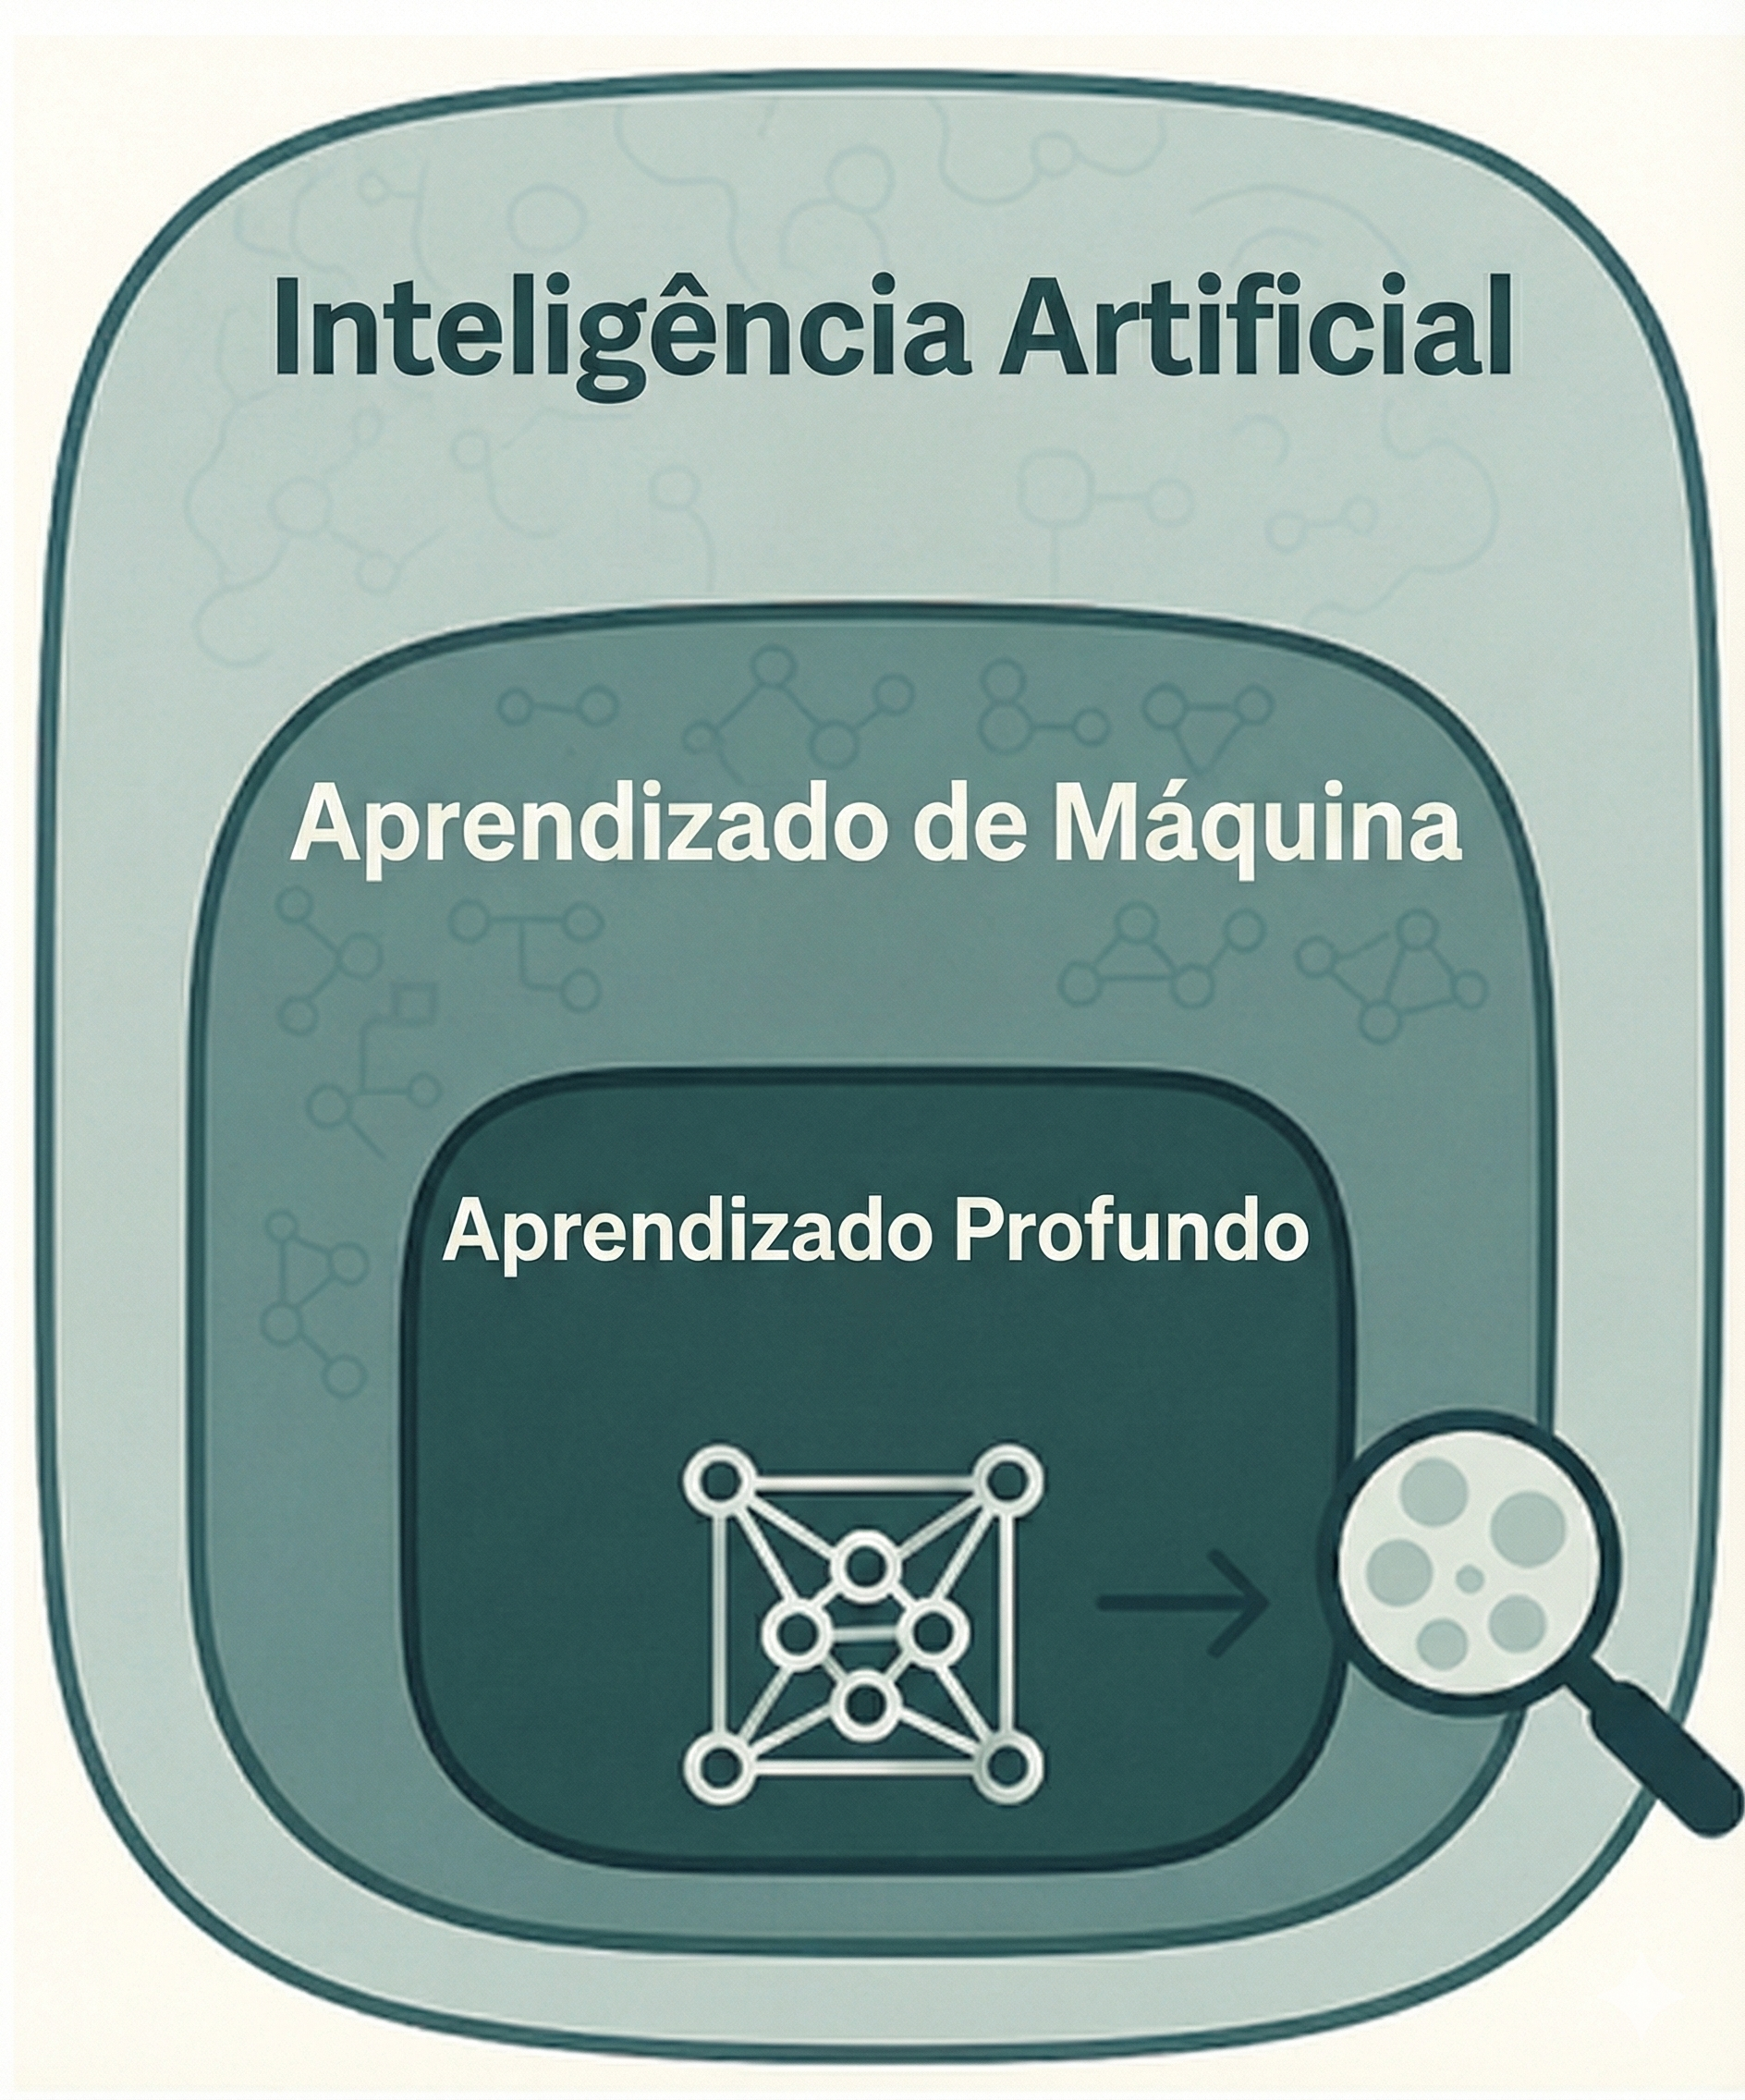
\includegraphics[width=0.6\textwidth]{figuras/AI_ML_DL.png} 
    \caption[Hierarquia Conceitual: IA, ML e DL]{Relação hierárquica entre Inteligência Artificial, Aprendizado de Máquina  e Aprendizado Profundo. Figura gerada pelo autor utilizando ferramenta de IA.}
    \label{fig:ia_ml_dl_hierarquia} 
\end{figure}

O DL utiliza múltiplas camadas de processamento interconectadas para aprender automaticamente representações hierárquicas de dados complexos \cite{Goodfellow2016, LeCun2015}. Diferentemente de abordagens de aprendizado de máquina tradicionais que frequentemente requerem uma etapa manual de extração de características (\textit{feature engineering}), os modelos de DL são capazes de aprender essas características diretamente dos dados brutos, como \textit{pixels} de uma imagem.

O funcionamento de uma rede neural em DL ocorre através de um processo cíclico e iterativo, composto essencialmente por quatro etapas principais que se repetem: a passagem de dados pela rede, o cálculo do erro, a identificação de onde ajustar e a atualização do modelo. Este fluxo está ilustrado na \Figura{fig:ciclo_treinamento_dl}.

% Figura do Ciclo de Treinamento DL Simplificado
\begin{figure}[!htb]
    \centering
    % Lembre-se de verificar se o nome do arquivo da imagem está correto
    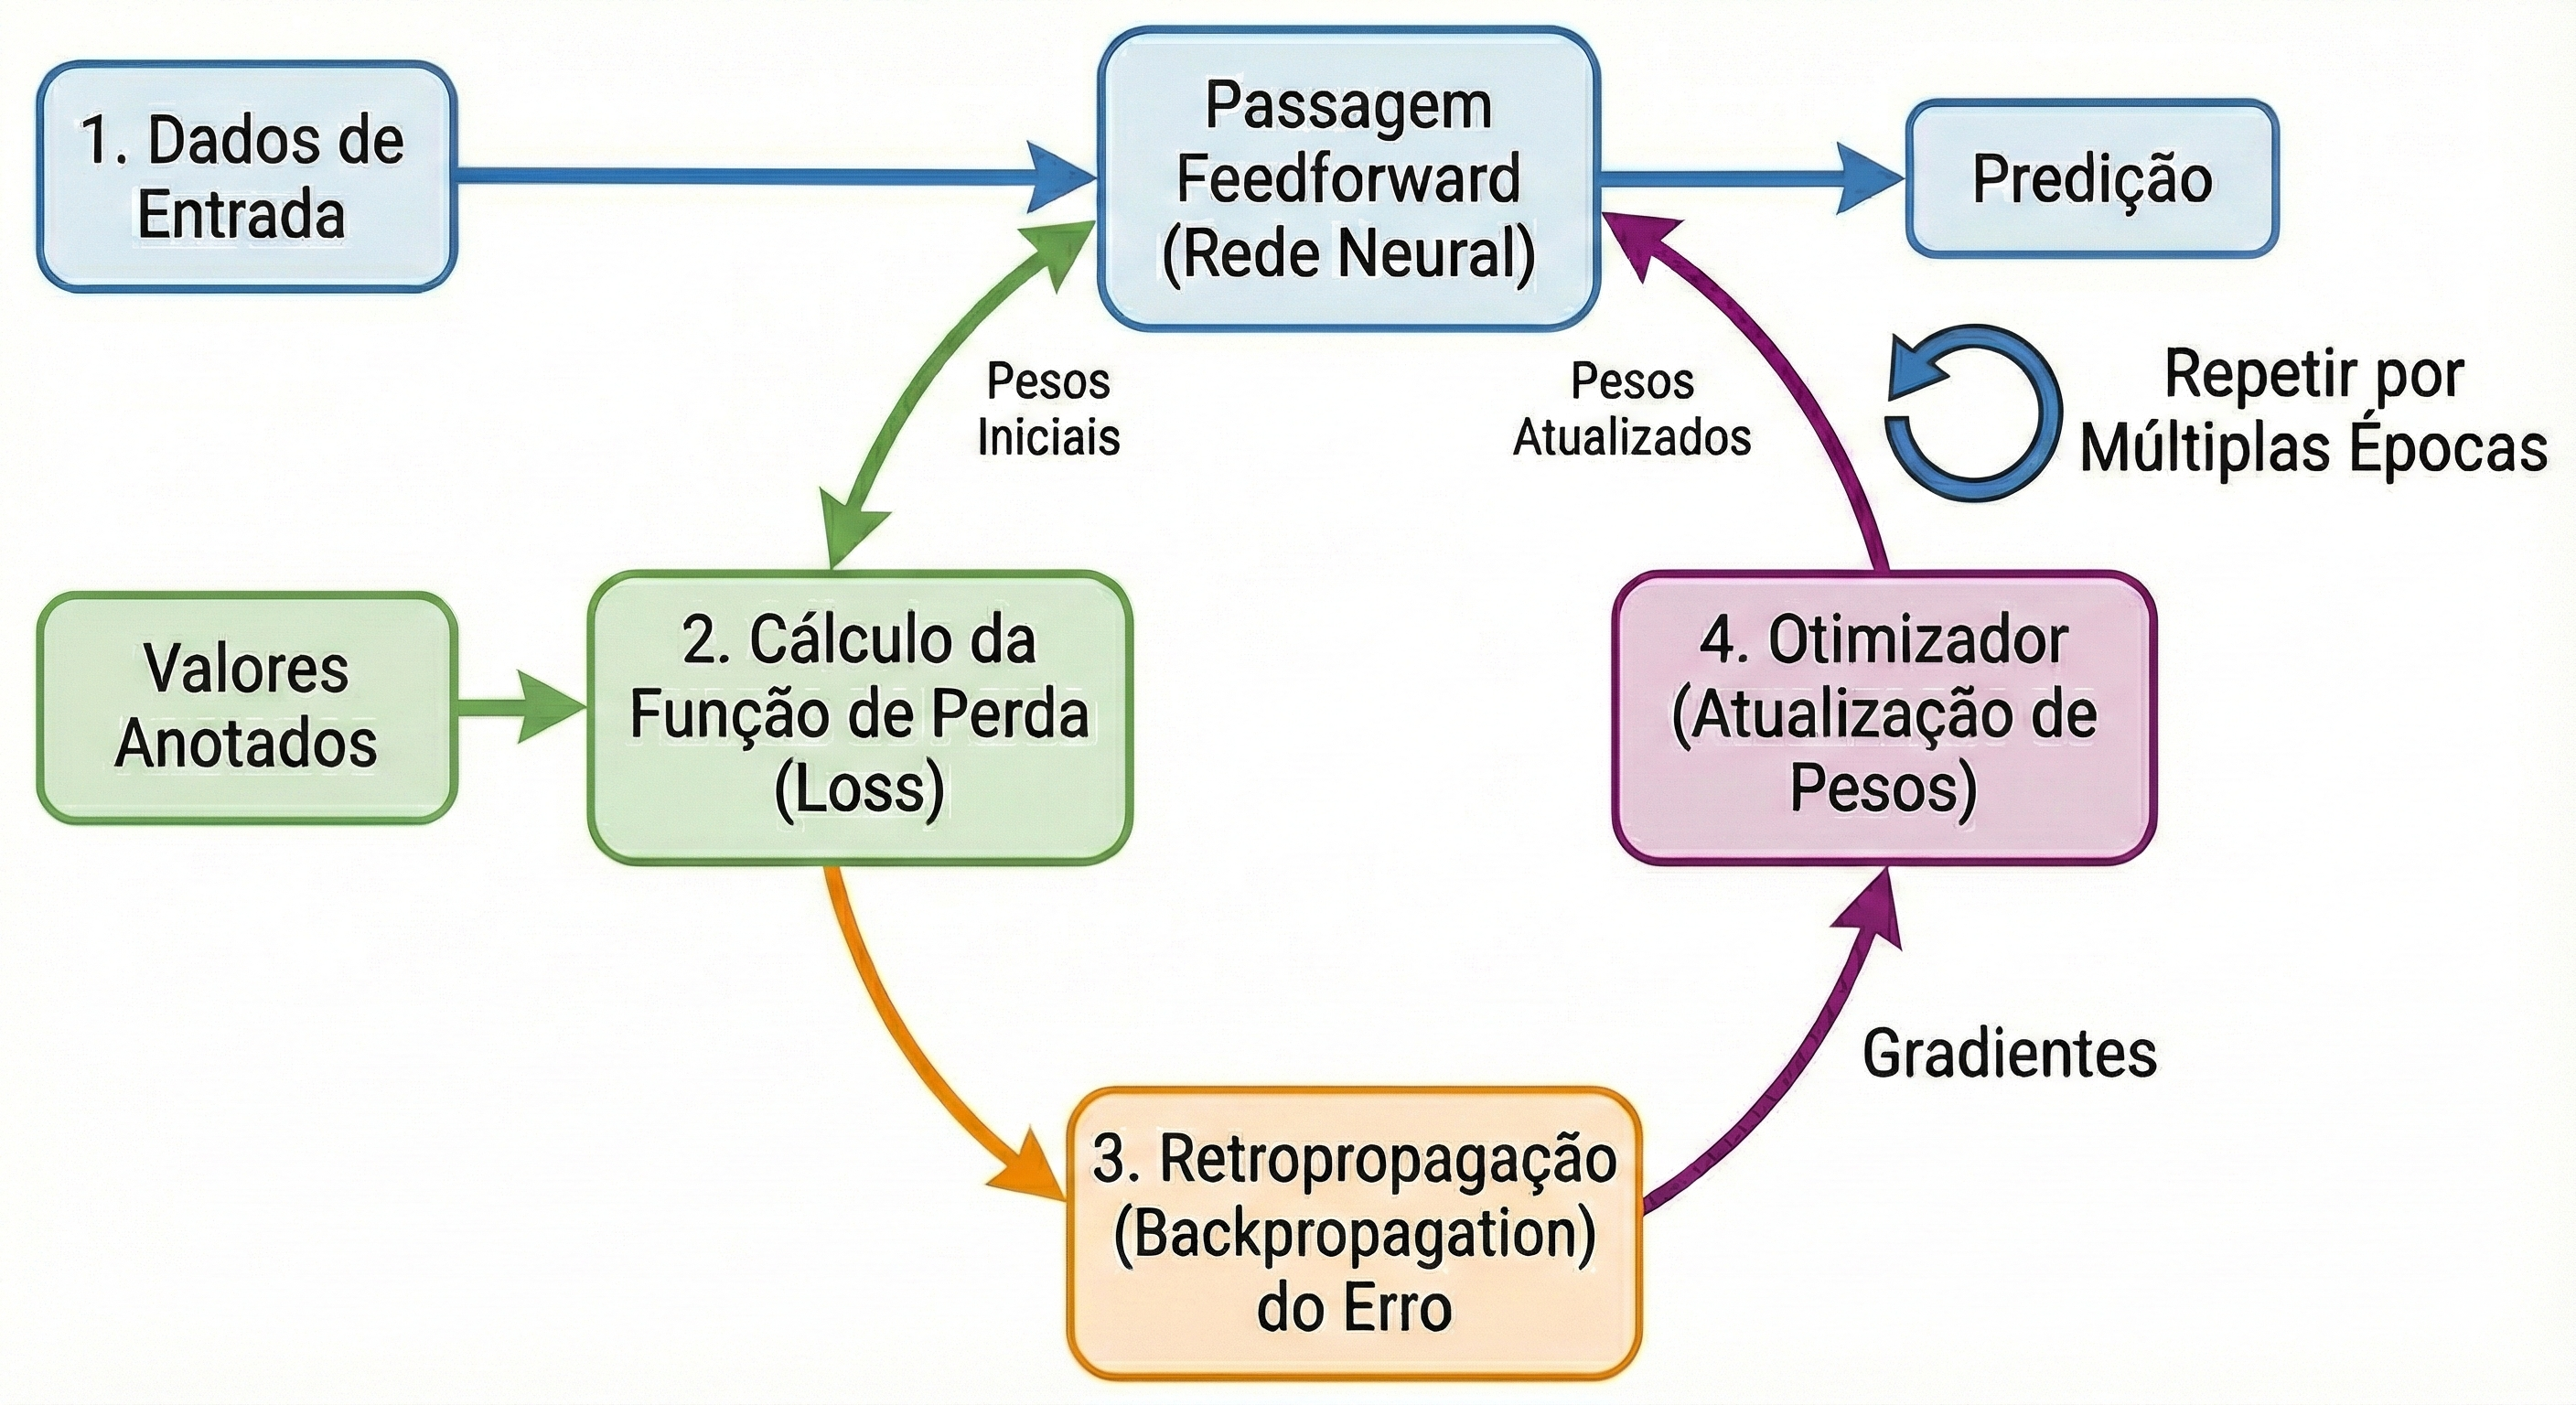
\includegraphics[width=0.8\textwidth]{figuras/DL_pipeline.png}
    \caption[Ciclo de Treinamento de um Modelo de Deep Learning.]{Diagrama esquemático do ciclo de treinamento de uma rede neural. Inicialmente, os dados de entrada são processados através da rede na passagem \textit{feedforward} para gerar uma predição. Em seguida, essa predição é comparada com os valores anotados (\textit{ground truth}) para calcular a função de perda (\textit{loss}). O erro resultante é então retropropagado via \textit{backpropagation} para calcular os gradientes, os quais são utilizados pelo otimizador para atualizar os pesos da rede. Este processo é repetido ciclicamente por múltiplas épocas. Figura gerada pelo autor utilizando ferramenta de IA.}
    \label{fig:ciclo_treinamento_dl}
\end{figure}

A primeira etapa é a propagação para frente (do inglês \textit{feedforward}). Nela, os \textbf{dados de entrada} são inseridos na rede neural e processados camada por camada. A rede utiliza seus parâmetros internos atuais (pesos) para transformar esses dados até gerar uma \textbf{predição} final.

Imediatamente após a predição, ocorre a avaliação de desempenho. O resultado gerado pela rede é comparado com os \textbf{valores anotados} (do inglês \textit{ground truth}), que representam a resposta correta esperada. A diferença entre o que a rede previu e o valor real é quantificada pela \textbf{função de perda} (do inglês \textit{loss}). Quanto maior o valor calculado nesta etapa, maior o erro cometido pelo modelo.

Para corrigir esse erro, o sistema executa a retropropagação (do inglês \textit{backpropagation}). O algoritmo analisa o erro final e percorre o caminho inverso na rede para calcular os \textbf{gradientes}. Conceitualmente, os gradientes indicam qual a direção e a intensidade do ajuste necessário em cada conexão da rede para diminuir o erro.

Por fim, o \textbf{otimizador} utiliza essas informações dos gradientes para efetivamente atualizar os pesos da rede. Com os pesos ajustados, o modelo está ligeiramente melhorado para a próxima rodada. Esse ciclo completo é repetido por múltiplas vezes (chamadas de épocas) até que a diferença entre a predição e os valores anotados seja minimizada a um nível aceitável.

No contexto da patologia digital, modelos de DL são treinados com grandes conjuntos de WSIs anotadas para identificar padrões sutis, muitas vezes imperceptíveis ao olho humano, que podem indicar a presença de câncer ou outras características patológicas.

\subsection{Anotações Médicas em Imagens e a Estrutura das WSIs}\label{subsec:anotacoes_estrutura_wsi}

O treinamento supervisionado de modelos de DL requer dados de referência, conhecidos como \textit{ground truth}. Em patologia digital, isso se traduz em anotações realizadas por patologistas experientes diretamente sobre as WSIs, delimitando ROIs, como áreas cancerosas e não cancerosas. % Referenciar Figura 5 e Figura 7 aqui, se ainda não estiverem em outro lugar próximo.
Essas anotações, frequentemente armazenadas em formatos como \Sigla{\textit{Extensible Markup Language}}{XML}, contêm as coordenadas dos polígonos que definem as ROIs e, por vezes, os códigos de cor utilizados para diferenciar as classes. A qualidade e a consistência dessas anotações são cruciais para o desempenho do modelo de DL.

Do ponto de vista computacional, uma WSI é uma imagem digital de grande escala, frequentemente na ordem de \textit{gigapixels}, composta por uma vasta matriz de \textit{pixels}, conforme ilustrado na \Figura{fig:wsi_pixel_patching_estrutura}. Cada pixel individual possui valores numéricos que representam a intensidade de cor, tipicamente nos canais Vermelho, Verde e Azul (do inglês \Sigla{\textit{Red, Green, Blue}}{RGB}), como detalhado no zoom da figura. A manipulação e análise eficientes desses dados massivos exigem estratégias de amostragem. Uma técnica fundamental nesse contexto é o \textit{patching}, onde a WSI é sistematicamente dividida em múltiplas sub-imagens menores, denominadas \textit{patches} (e.g., 224x224 \textit{pixels}). Esses \textit{patches}, também representados na \Figura{fig:wsi_pixel_patching_estrutura}, são então utilizados como entrada para os modelos de DL para tarefas como a segmentação semântica. A metodologia de \textit{patching} empregada neste trabalho é detalhada na \Secao{sec:met_corte_imagens} e o resultado quantitativo da geração de \textit{patches} é apresentado na \Secao{sec:res_dataset_base}.

% Figura da Estrutura da WSI e Patching
\begin{figure}[!htb]
    \centering
    % Substitua 'figuras/wsi_structure_patching.png' pelo nome/caminho correto da sua nova imagem
    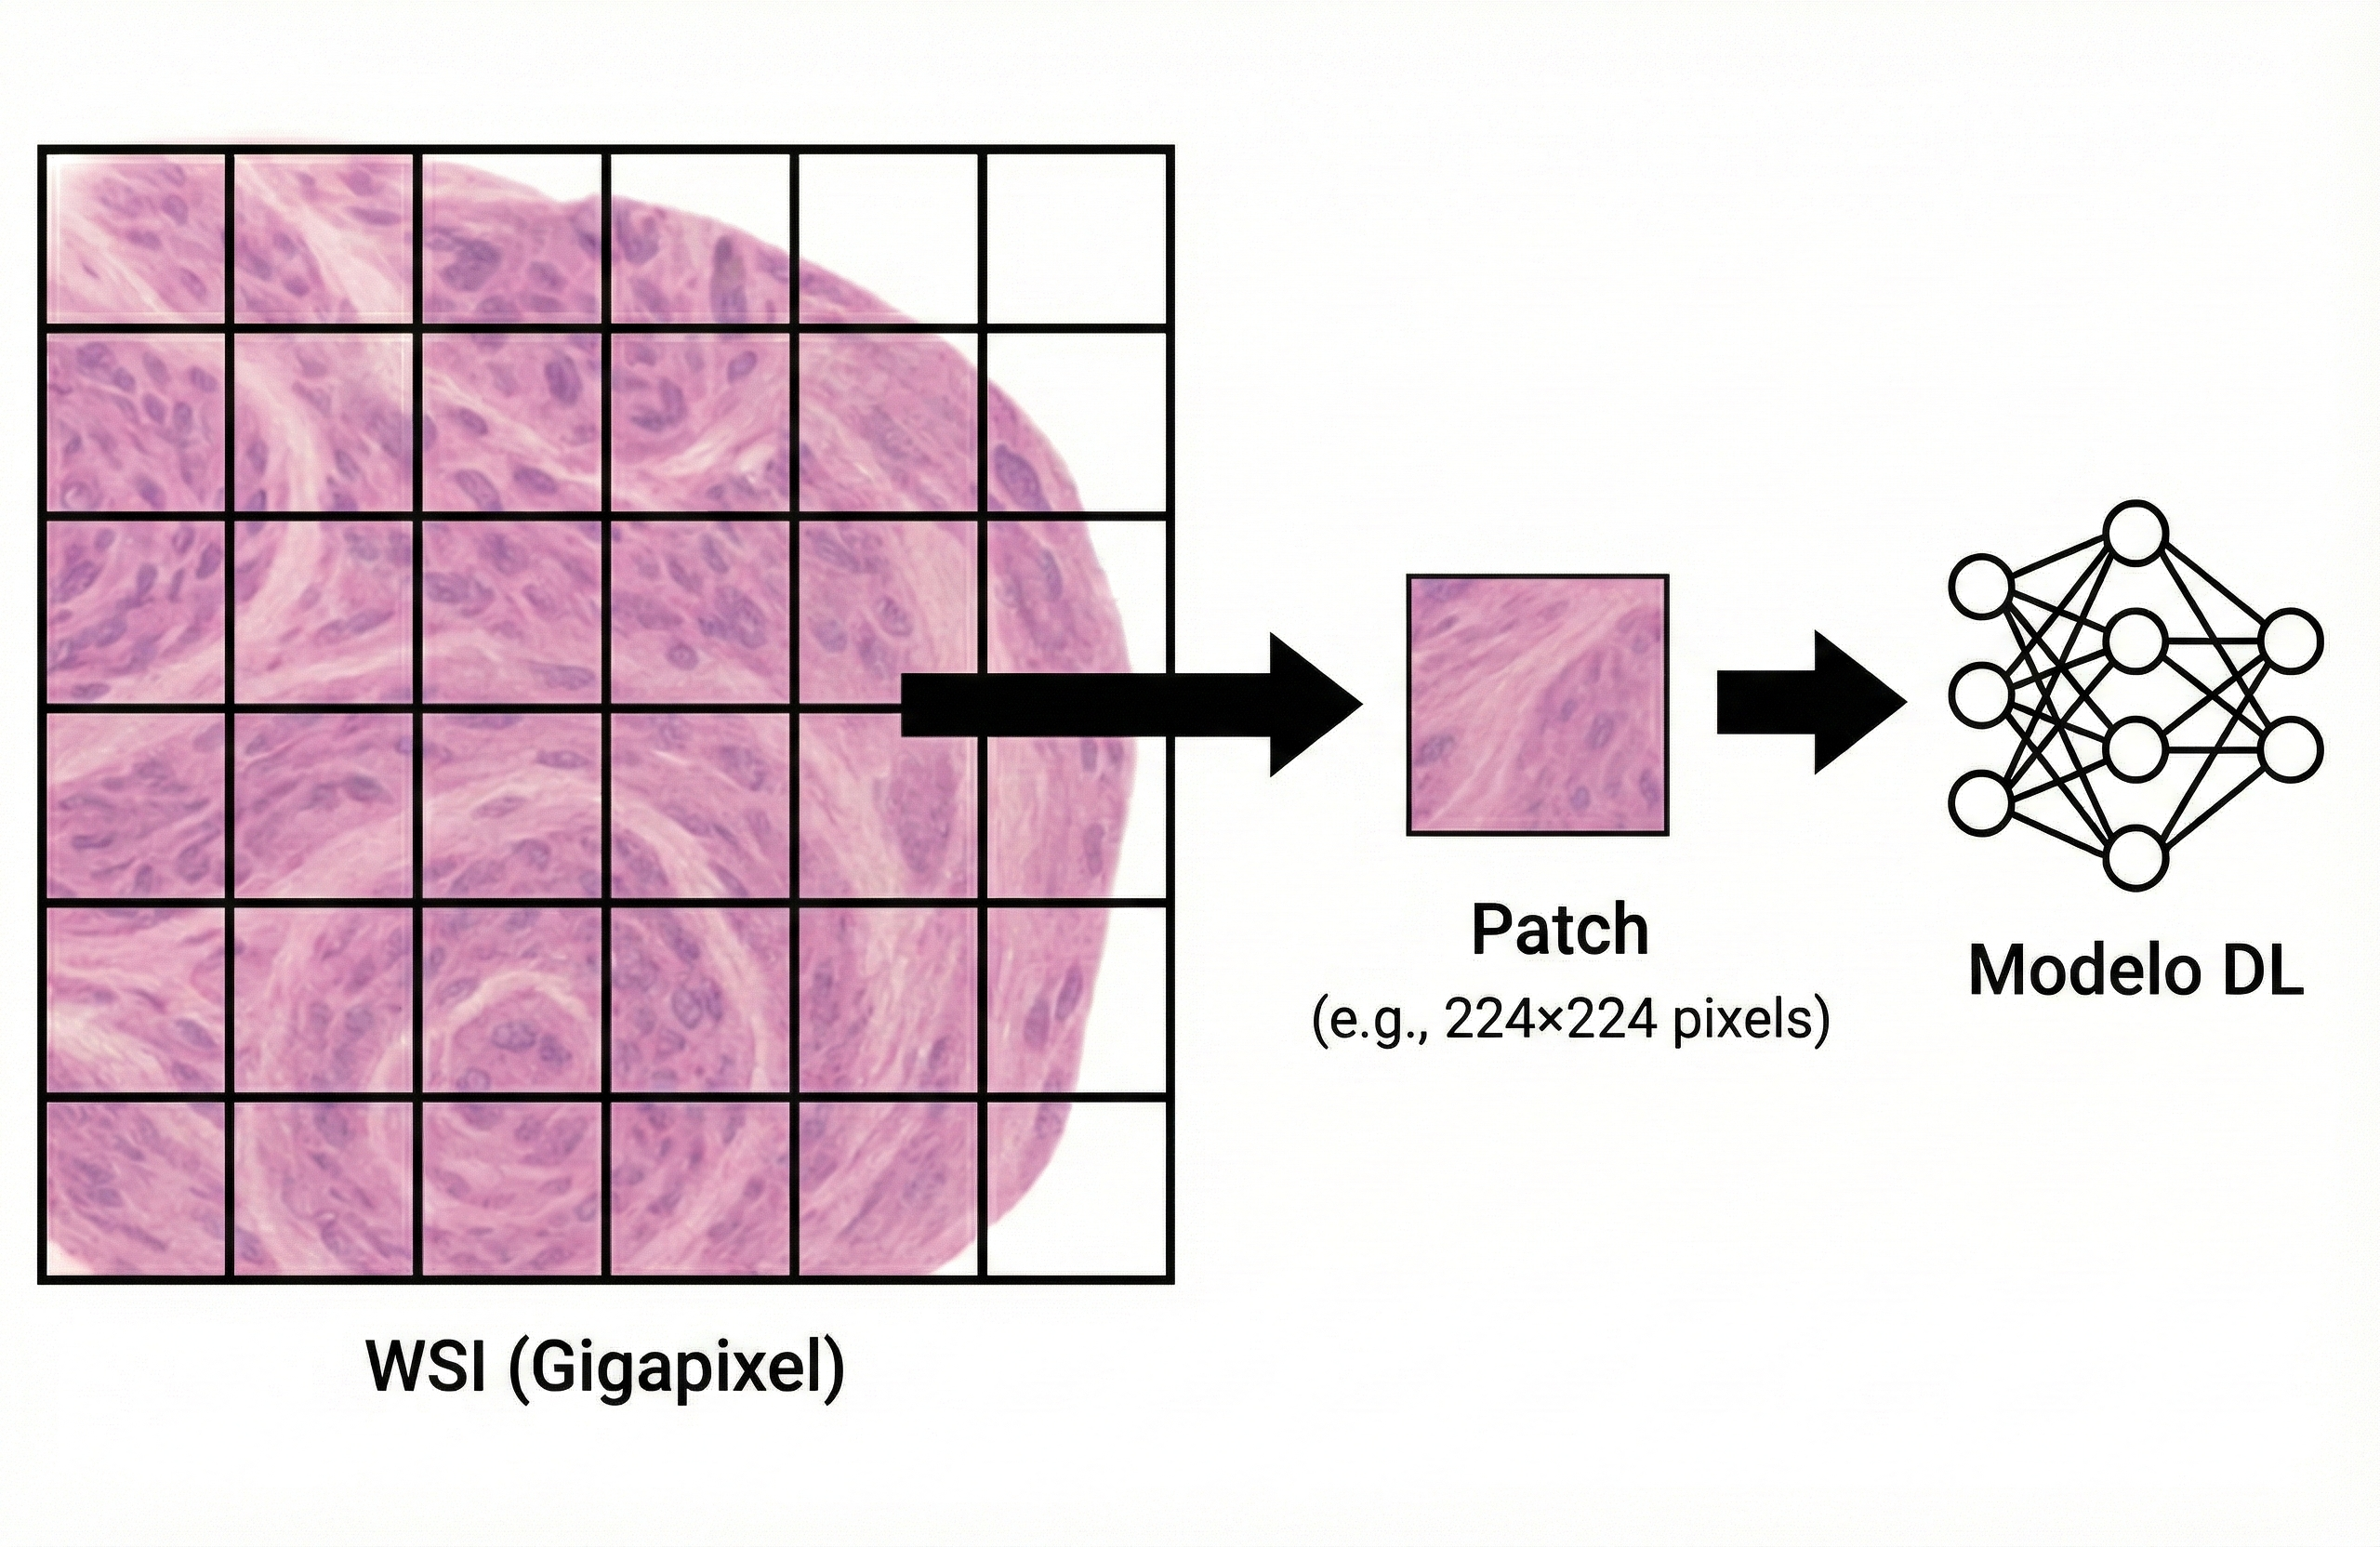
\includegraphics[width=0.9\textwidth]{figuras/WSI_schema.png}
    \caption[Estrutura de uma WSI e o Conceito de \textit{Patching}]{Ilustração simplificada do processo de \textit{patching}. À esquerda, a WSI em escala de \textit{gigapixel} é sobreposta por uma grade de segmentação. A seta indica a extração de um único \textit{patch} (e.g., 224x224 \textit{pixels}), que serve como entrada para o modelo de DL (representado esquematicamente). Figura gerada pelo autor utilizando ferramenta de IA.}
    \label{fig:wsi_pixel_patching_estrutura}
\end{figure}

\subsection{Pré-processamento de Imagens em Patologia Digital}\label{subsec:preprocessamento_patologia}

Antes que as WSIs ou seus \textit{patches} possam ser utilizados efetivamente para treinar modelos de DL, uma série de etapas de pré-processamento são recomendadas para padronizar os dados, mitigar artefatos e realçar características relevantes. Artefatos, neste contexto, referem-se a imperfeições ou distorções presentes em imagens médicas digitais que não correspondem às estruturas biológicas originais, sendo frequentemente introduzidos por fatores como variações no preparo das lâminas, coloração, digitalização ou compressão da imagem \cite{Jurgas2024}. Estas etapas de pré-processamento visam tornar o processo de aprendizado mais robusto e generalizável.

\subsubsection{Segmentação de Tecido e Refinamento Morfológico}\label{subsubsec:fund_segmentacao_tecido}

As WSIs frequentemente contêm grandes áreas de fundo branco (correspondentes ao vidro da lâmina) que não possuem informação diagnóstica relevante e podem enviesar o treinamento dos modelos. Portanto, uma etapa inicial fundamental é a \textbf{Segmentação de Tecido}, que visa distinguir as regiões que contêm tecido biológico do fundo da imagem. Para isso, frequentemente se explora a diferença de características entre essas regiões, como a saturação de cor. No espaço de cor HSV (\textit{Hue, Saturation, Value}), o canal de saturação (S) costuma apresentar valores mais altos nas regiões de tecido corado em comparação com o fundo acromático.

Uma abordagem comum para limiarizar automaticamente o canal de saturação (ou outra representação da imagem, como escala de cinza) é o \textbf{Método de Otsu} \cite{Otsu1979}. Este método calcula um limiar ótimo ($t$) analisando o histograma de intensidades dos \textit{pixels}. O limiar $t$ é escolhido de forma a separar os \textit{pixels} em duas classes (fundo e tecido) de maneira que os \textit{pixels} dentro de cada classe sejam o mais homogêneos possível (ou seja, tenham baixa variância interna) e, ao mesmo tempo, que as duas classes sejam o mais distintas possível uma da outra. A limiarização de Otsu pode ser representada como:
\begin{equation}\label{eq:otsu_threshold}
    g(x,y) = \begin{cases} 
      1 & \text{se } f(x,y) > t \\
      0 & \text{se } f(x,y) \leq t 
   \end{cases}
\end{equation}
onde $f(x,y)$ é o valor do pixel na imagem de entrada (\eg, canal de saturação) e $g(x,y)$ é a máscara binária resultante. Embora eficaz, variações na iluminação podem requerer abordagens adaptativas.

A máscara binária resultante da limiarização pode conter ruídos. Para refinar esta máscara, aplicam-se \textbf{Transformações Morfológicas} \cite{Gonzalez2006}, que são operações baseadas em teoria de conjuntos aplicadas à estrutura da imagem usando um elemento estruturante (kernel). As duas operações fundamentais são a erosão ($\ominus$) e a dilatação ($\oplus$), que, quando combinadas, formam operações mais complexas como Abertura ($A \circ B = (A \ominus B) \oplus B$) e Fechamento ($A \bullet B = (A \oplus B) \ominus B$). A aplicação sequencial de Abertura e Fechamento é uma estratégia comum para um refinamento robusto da máscara de tecido, removendo ruídos e preenchendo pequenos buracos, como ilustrado na \Figura{fig:abertura_fechamento_morfologico}.

\begin{figure}[!htb]
    \centering
    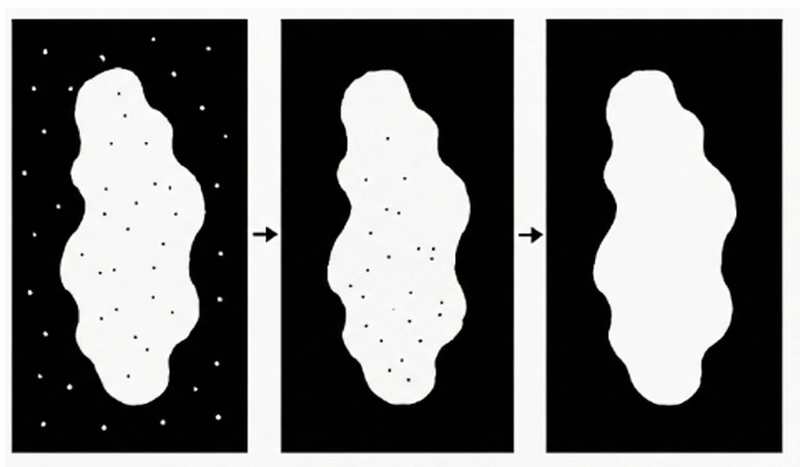
\includegraphics[width=0.8\textwidth]{figuras/morphological_operation.png}
    \caption[Efeito Sequencial das Operações Morfológicas de Abertura e Fechamento]{Ilustração do efeito da aplicação sequencial de operações morfológicas. \textbf{(Esquerda)} Máscara binária ruidosa de entrada. \textbf{(Centro)} Resultado após a aplicação da operação de Abertura, que remove o ruído externo. \textbf{(Direita)} Resultado final após a aplicação da operação de Fechamento sobre a máscara já aberta, preenchendo os buracos internos e resultando em uma região de interesse mais coesa. Figura gerada pelo autor utilizando ferramenta de IA.}
    \label{fig:abertura_fechamento_morfologico}
\end{figure}

% --- PARÁGRAFO DE TRANSIÇÃO E NOVO CONTEÚDO ---
Além das abordagens baseadas em limiarização global e refinamento local, métodos de segmentação mais avançados, como os baseados em grafos, oferecem uma solução mais robusta e adaptativa.

Uma abordagem alternativa e poderosa para segmentação é a proposta por \textcite{Felzenszwalb2004}, baseada em grafos. Neste método, a imagem é representada como um grafo não direcionado $G=(V, E)$, onde cada \textit{pixel} é um vértice em $V$ e uma aresta em $E$ conecta pares de \textit{pixels} vizinhos. A cada aresta $(v_i, v_j)$ é atribuído um peso $w(v_i, v_j)$ que representa a dissimilaridade entre os \textit{pixels} (\eg, a diferença em intensidade ou cor).

O algoritmo segmenta a imagem ao particionar os vértices em um conjunto de componentes conectados $S$. A decisão de fundir (ou não) dois componentes se baseia em um predicado que compara a dissimilaridade entre os componentes com a dissimilaridade interna de cada um. A \textbf{diferença interna} de um componente $C$, denotada por $Int(C)$, é definida como o maior peso de aresta na árvore geradora mínima (MST) de $C$:
\begin{equation}
    Int(C) = \max_{e \in \text{MST}(C,E)} w(e)
\end{equation}
Essa medida representa a maior dissimilaridade \textit{dentro} de uma região. Por sua vez, a diferença entre dois componentes $C_1$ e $C_2$, $Dif(C_1, C_2)$, é o menor peso de aresta que os conecta:
\begin{equation}
    Dif(C_1, C_2) = \min_{v_i \in C_1, v_j \in C_2, (v_i, v_j) \in E} w(v_i, v_j)
\end{equation}
O algoritmo então funde dois componentes se a diferença entre eles ($Dif$) não for significativamente maior que a diferença interna de ambos. Formalmente, uma fronteira entre $C_1$ e $C_2$ é mantida se $Dif(C_1, C_2)$ for maior que a diferença interna mínima dos componentes, $MInt(C_1, C_2)$, definida como:
\begin{equation}
    MInt(C_1, C_2) = \min(Int(C_1) + \tau(C_1), Int(C_2) + \tau(C_2))
\end{equation}
onde $\tau(C) = k/|C|$ é uma função de limiar que depende do tamanho do componente $|C|$. O parâmetro $k$ controla a escala da segmentação: um $k$ maior favorece a criação de segmentos maiores. Essa formulação permite que o método seja adaptativo, preservando detalhes em regiões de baixa variação enquanto ignora variações em regiões de alta textura, tornando-o particularmente adequado para a complexidade das imagens histopatológicas.

% Figura Ilustrativa do Processo de Segmentação de Tecido Baseada em Grafos
\begin{figure}[!htb] 
    \centering
    % Garanta que o arquivo 'graph_segmentation_wsi_process.png' esteja na sua pasta de figuras.
    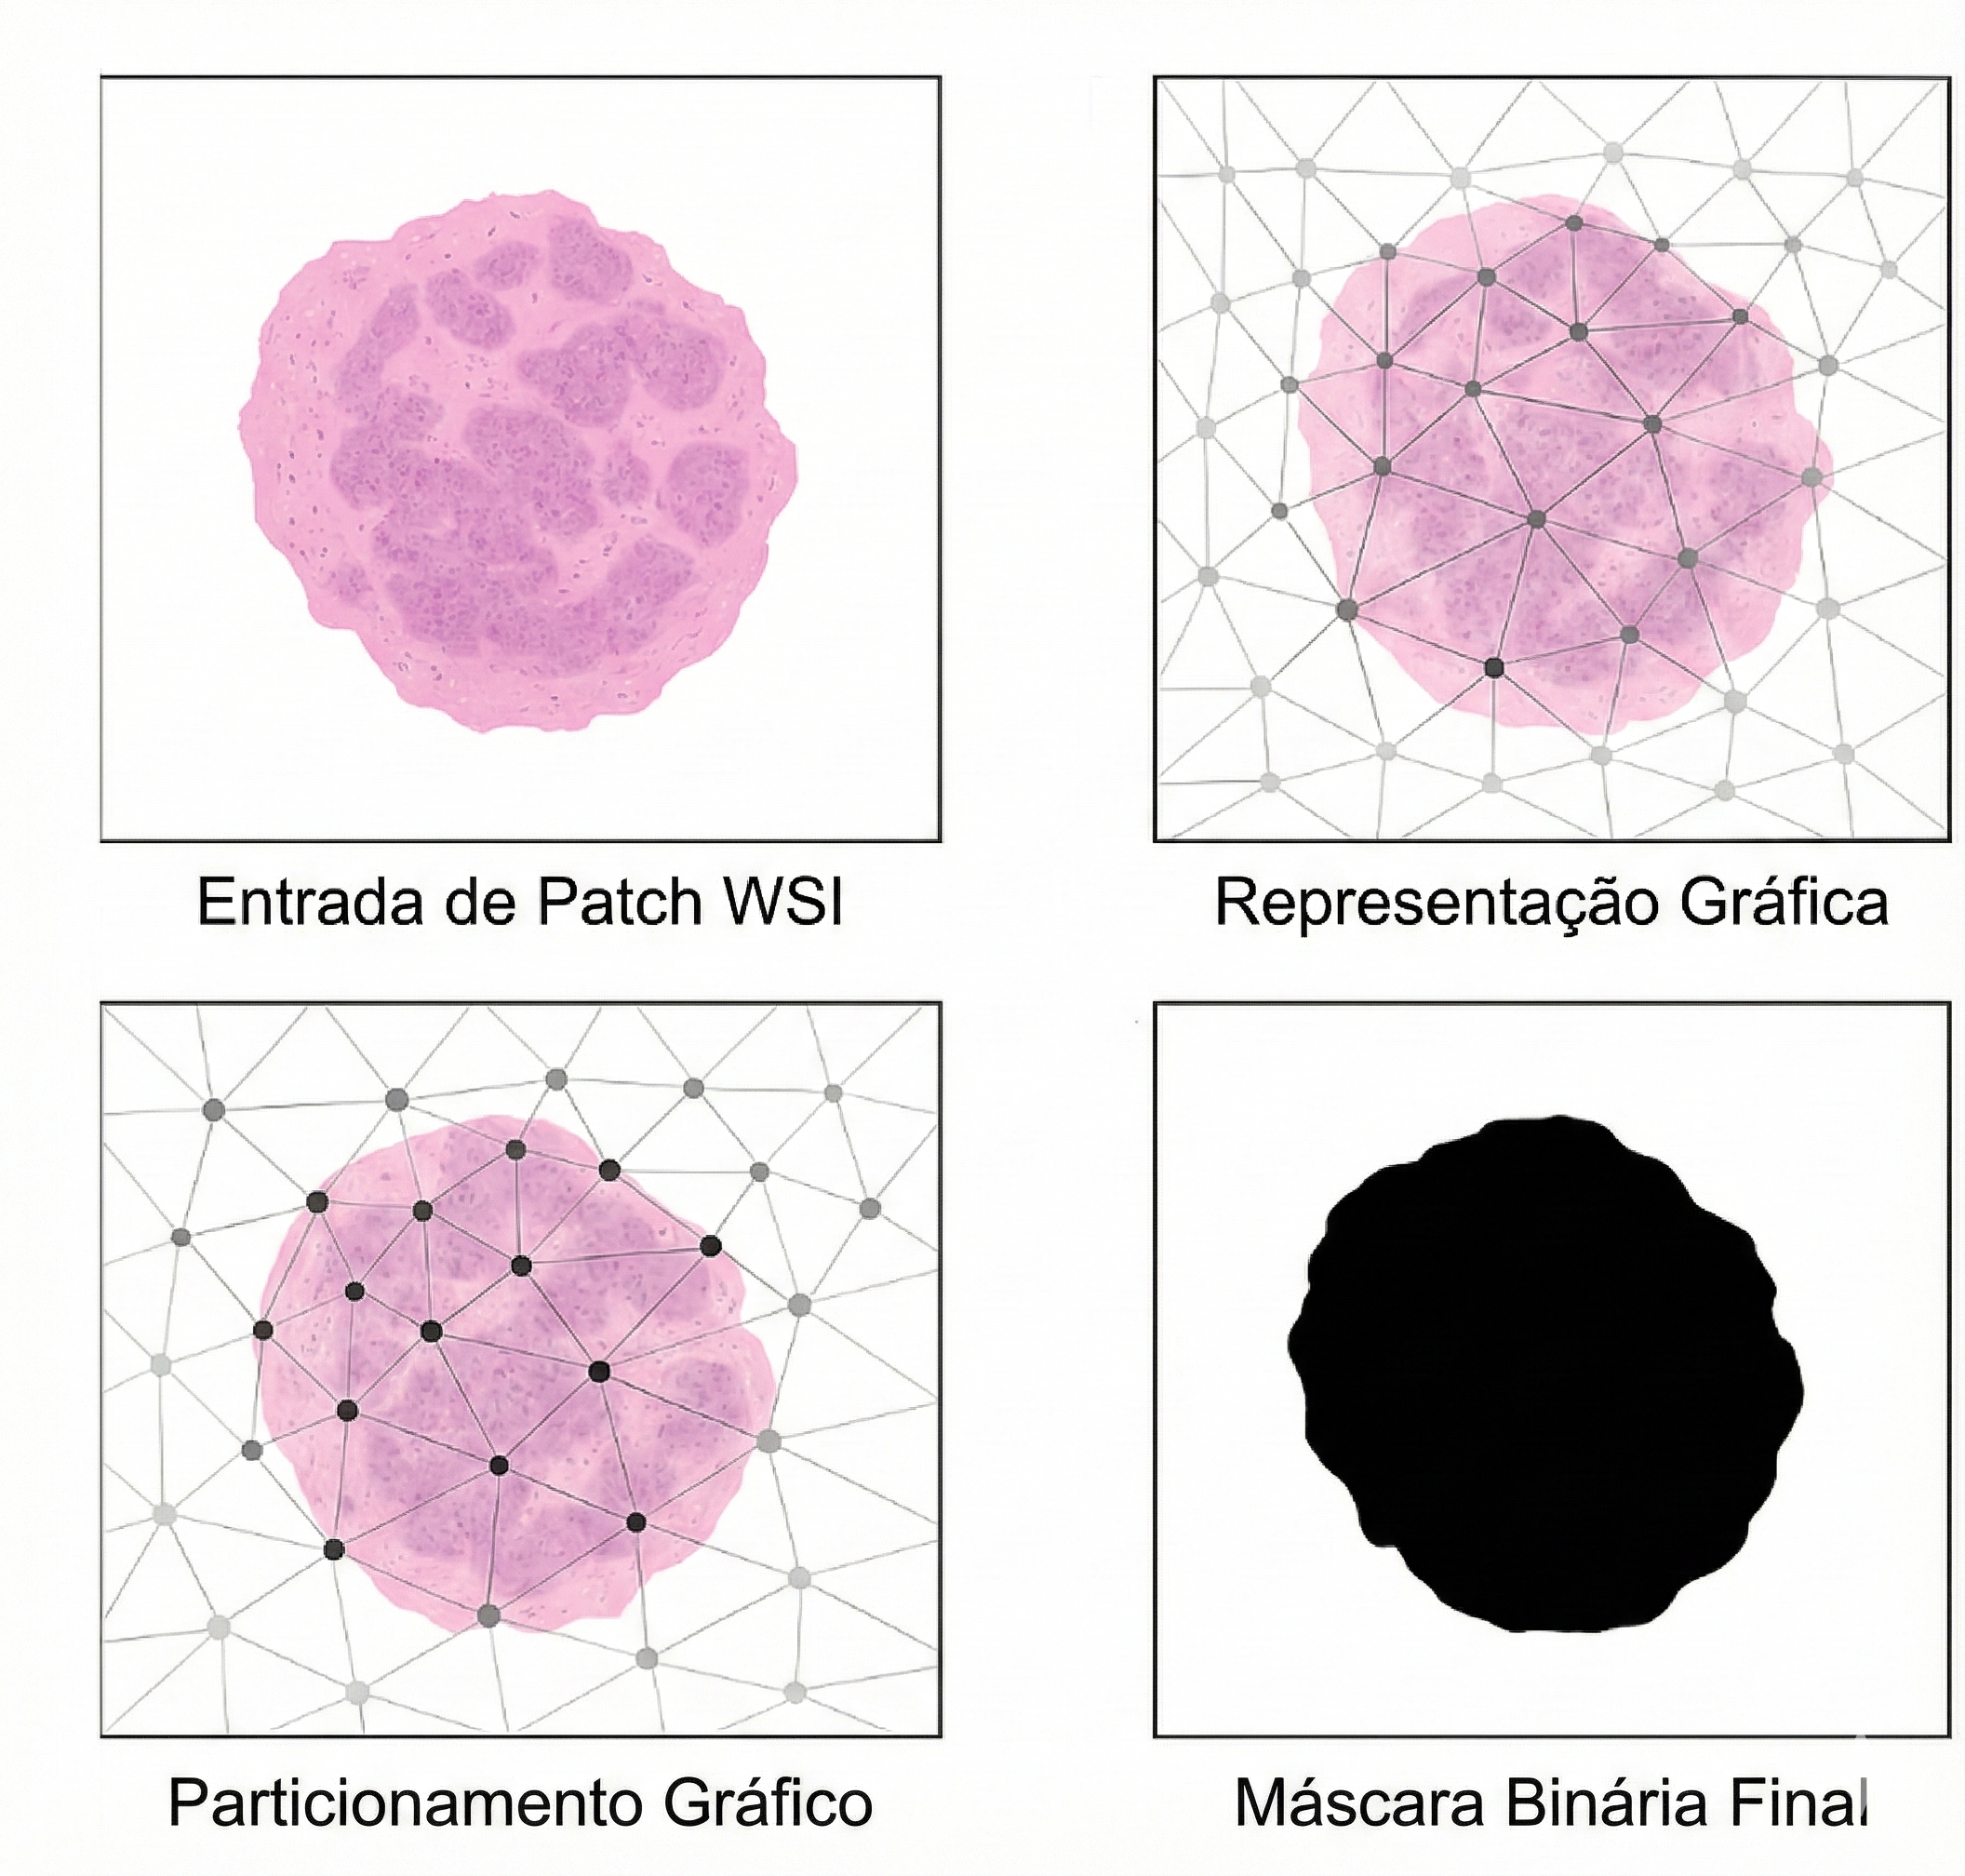
\includegraphics[width=0.95\textwidth]{figuras/graph_method.png} 
    \caption[Ilustração do Processo de Segmentação de Tecido Baseada em Grafos]{Ilustração do processo de segmentação de tecido em uma WSI utilizando uma abordagem baseada em grafos. 
    \textbf{(Superior Esquerdo)} \textit{Patch} de entrada contendo tecido (rosa/roxo) e fundo (branco). 
    \textbf{(Superior Direito)} A imagem é convertida em um grafo, onde os pesos das arestas (espessura das linhas) são altos na interface tecido-fundo. 
    \textbf{(Inferior Esquerdo)} O algoritmo particiona o grafo em componentes (tecido vs. fundo), "cortando" as arestas de alto peso. 
    \textbf{(Inferior Direito)} O resultado é uma máscara binária, onde o tecido detectado é representado em preto e o fundo em branco, servindo como entrada para as etapas subsequentes de análise. Figura gerada pelo autor
utilizando ferramenta de IA.}
    \label{fig:graph_segmentation_wsi_illustration} 
\end{figure}

\subsubsection{Normalização de Cor}\label{subsubsec:fund_norm_cor}

A variabilidade na coloração Hematoxilina e Eosina (H\&E) entre diferentes lâminas histológicas é um desafio proeminente em patologia digital, podendo ser introduzida por diversos fatores no preparo ou digitalização \cite{Xiong2021StainVariability}. Esta inconsistência pode confundir modelos de \textit{deep learning}, que podem interpretar variações de cor como diferenças biológicas, prejudicando sua capacidade de generalização. Para mitigar esse problema, diversas técnicas de normalização de cor foram propostas, variando de abordagens estatísticas a métodos baseados em deconvolução de cor.

\paragraph{Normalização por Mapeamento Estatístico (Reinhard et al.)}
Uma técnica de normalização de cor amplamente adotada é a proposta por \textcite{Reinhard2001}. O método opera no espaço de cor CIE LAB \cite{CIE2004} – que desacopla a luminosidade (L*) da cromaticidade (canais a* e b*) – ajustando a média ($\mu_{origem}$) e o desvio padrão ($\sigma_{origem}$) de cada canal da imagem de origem para que correspondam aos de uma referência ($\mu_{ref}, \sigma_{ref}$). A transformação para cada pixel $P_{LAB, origem}$ é dada por:
\begin{equation}\label{eq:reinhard_norm_fund}
    P_{LAB, norm} = \left( \frac{\sigma_{ref}}{\sigma_{origem}} \right) (P_{LAB, origem} - \mu_{origem}) + \mu_{ref}
\end{equation}
Apesar de sua simplicidade e eficácia, essa abordagem trata a imagem de forma global, sem modelar explicitamente a contribuição de cada corante individualmente.

\paragraph{Normalização por Deconvolução de Cor (Ruifrok et al.)}
Métodos baseados em deconvolução de cor buscam separar a contribuição de cada corante (e.g., Hematoxilina e Eosina) na imagem. A abordagem de \textcite{Ruifrok2001} fundamenta-se na lei de Beer-Lambert \textcite{BeerLambert1962}, que estabelece uma relação linear entre a concentração do corante e a Densidade Óptica (do inglês \Sigla{\textit{Optical Density}}{OD}), e não a intensidade RGB. A conversão de RGB para OD é geralmente feita por:
\begin{equation}
    OD = -\log_{10}\left(\frac{I}{I_0}\right)
\end{equation}
onde $I$ é a intensidade da luz transmitida e $I_0$ é a intensidade da luz incidente.
Este método utiliza uma matriz de deconvolução de cor, previamente definida a partir de amostras puras de cada corante, para separar as imagens RGB em canais que representam a concentração de cada um. Uma vez separadas, as imagens podem ser reconstruídas utilizando uma matriz de coloração de referência, padronizando a aparência. A principal limitação é a necessidade de uma matriz de corantes fixa e bem calibrada, que pode não se generalizar para todas as variações de preparo de lâminas.

\paragraph{Normalização Adaptativa por Deconvolução de Cor (Macenko et al.)}
Para superar a necessidade de uma matriz de corantes pré-definida, \textcite{Macenko2009} propuseram um método que estima os vetores de coloração diretamente de cada imagem. O processo também se inicia com a conversão do espaço RGB para OD. Em seguida, aplica-se a \Sigla{\textit{Singular Vector Decomposition}}{SVD} sobre os valores de OD dos \textit{pixels} (após remover \textit{pixels} de fundo). A SVD identifica as direções de maior variação no espaço de cor, que correspondem aos vetores de cada corante.
Uma vez que os vetores de coloração da imagem de origem e da imagem de referência são determinados, as concentrações de corante na imagem de origem são calculadas e, então, a imagem é reconstruída usando os vetores de cor da referência. A natureza adaptativa deste método o torna robusto a diferentes condições de coloração.

\paragraph{Normalização com Preservação de Estrutura (Vahadane et al.)}
Uma evolução das técnicas de deconvolução foi proposta por \textcite{Vahadane2016}, que introduziram o uso de \Sigla{\textit{Sparse Non-negative Matrix Factorization}}{SNMF} para a separação dos corantes. Esta abordagem é motivada por duas propriedades físicas e biológicas: (i) a concentração de corantes não pode ser negativa (não-negatividade) e (ii) em qualquer ponto da imagem, o pixel é tipicamente dominado por um único corante — por exemplo, o núcleo pela Hematoxilina ou o citoplasma pela Eosina (esparsidade).
O método modela a matriz de OD ($V$) como o produto de uma matriz de vetores de corante ($W$) e uma matriz de concentração de corantes ($H$), resolvendo o seguinte problema de otimização:
\begin{equation}
    \min_{W,H} \frac{1}{2} \|V - WH\|_F^2 + \lambda \|H\|_1, \quad \text{sujeito a} \quad W, H \ge 0
\end{equation}
onde $\lambda$ é o parâmetro que controla a esparsidade. Ao forçar a esparsidade, o método tende a preservar melhor a estrutura e a textura do tecido, evitando artefatos que podem surgir em outras técnicas. A normalização ocorre ao se substituir a matriz $W$ da imagem de origem pela matriz $W_{ref}$ da imagem de referência para reconstruir a imagem normalizada.

% Figura Comparativa dos Métodos de Normalização de Cor (Layout 2+2+1)
\begin{figure}[!htb]
    \centering % Centraliza todo o conteúdo da figura na página
    
    % --- PRIMEIRA LINHA ---
    \begin{subfigure}[b]{0.48\textwidth}
        \centering
        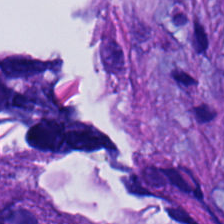
\includegraphics[width=0.8\linewidth]{figuras/original_patch.png}
        \caption{Patch Original}
        \label{fig:norm_original_2c}
    \end{subfigure}
    \hfill % Espaçamento horizontal flexível
    \begin{subfigure}[b]{0.48\textwidth}
        \centering
        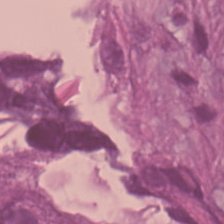
\includegraphics[width=0.8\linewidth]{figuras/reinhard_patch.png}
        \caption{Após Normalização (Reinhard)}
        \label{fig:norm_reinhard_2c}
    \end{subfigure}
    
    % --- SEGUNDA LINHA ---
    \begin{subfigure}[b]{0.48\textwidth}
        \centering
        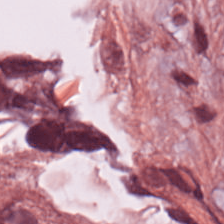
\includegraphics[width=0.8\linewidth]{figuras/macenko_patch.png}
        \caption{Após Normalização (Macenko)}
        \label{fig:norm_macenko_2c}
    \end{subfigure}
    \hfill
    \begin{subfigure}[b]{0.48\textwidth}
        \centering
        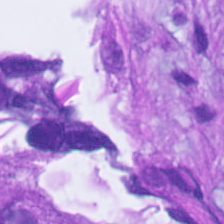
\includegraphics[width=0.8\linewidth]{figuras/ruifrok_patch.png}
        \caption{Após Normalização (Ruifrok)}
        \label{fig:norm_ruifrok_2c}
    \end{subfigure}

    % --- TERCEIRA LINHA (IMAGEM ÚNICA CENTRALIZADA) ---
    \begin{subfigure}[b]{0.48\textwidth}
        \centering
        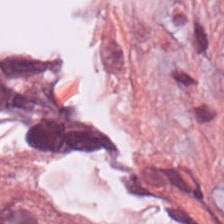
\includegraphics[width=0.8\linewidth]{figuras/vahadane_patch.png}
        \caption{Após Normalização (Vahadane)}
        \label{fig:norm_vahadane_2c}
    \end{subfigure}

    \caption[Comparação de Métodos de Normalização de Cor.]{Comparação visual de um \textit{patch} de WSI original (a) com os resultados das diferentes técnicas de normalização de cor aplicadas: (b) Reinhard, (c) Macenko, (d) Ruifrok e (e) Vahadane. A disposição em múltiplas linhas facilita a comparação dos resultados, com destaque para a preservação de estrutura nos métodos baseados em deconvolução de cor (c, d, e).}
    \label{fig:normalizacao_comparacao_2x2x1}
\end{figure}


\subsection{Segmentação Semântica}\label{subsec:segmentacao_semantica}

A \textbf{Segmentação Semântica} é a tarefa central abordada nesta dissertação. Para compreendê-la adequadamente, é essencial estabelecer primeiramente uma distinção clara em relação à classificação de imagens. A classificação é um processo global, cujo objetivo é atribuir um único rótulo ou categoria a toda a imagem de entrada, indicando apenas o objeto ou cena predominante \cite{Deng2009}.

Em contrapartida, a segmentação é uma tarefa inerentemente espacial e densa. Conforme definido por \textcite{Gonzalez2006}, o objetivo geral da segmentação é particionar uma imagem em suas regiões constituintes ou objetos. Na abordagem da segmentação semântica, isso se traduz na classificação de cada \textit{pixel} individual da imagem em uma categoria específica, preservando a localização espacial da informação \cite{Long2015}. Isso difere, inclusive, da detecção de objetos, que apenas localiza instâncias com caixas delimitadoras ( as chamadas \textit{bounding boxes}), sem definir seus contornos exatos\cite{Ren2015}.

No contexto específico deste trabalho, o foco recai sobre a segmentação semântica binária. O objetivo é classificar os \textit{pixels} em apenas duas categorias distintas (\eg, "objeto de interesse" \textit{versus} "fundo"). Em patologia digital, essa abordagem permite a delineação precisa e granular de regiões tumorais (\eg, tecidos classificados como "câncer" ou "não câncer"). Esse nível de detalhe fornece informações valiosas para a quantificação da extensão da doença e análise morfológica, conforme ilustrado na Figura \ref{fig:segmentacao_semantica_exemplo}.

\begin{figure}[!htb] % Sugestão de posicionamento: aqui, topo ou fundo.
    \centering
    % Comando para incluir sua imagem de segmentação semântica
    % Substitua 'nome_arquivo_segmentacao.png' pelo nome do seu arquivo de imagem
    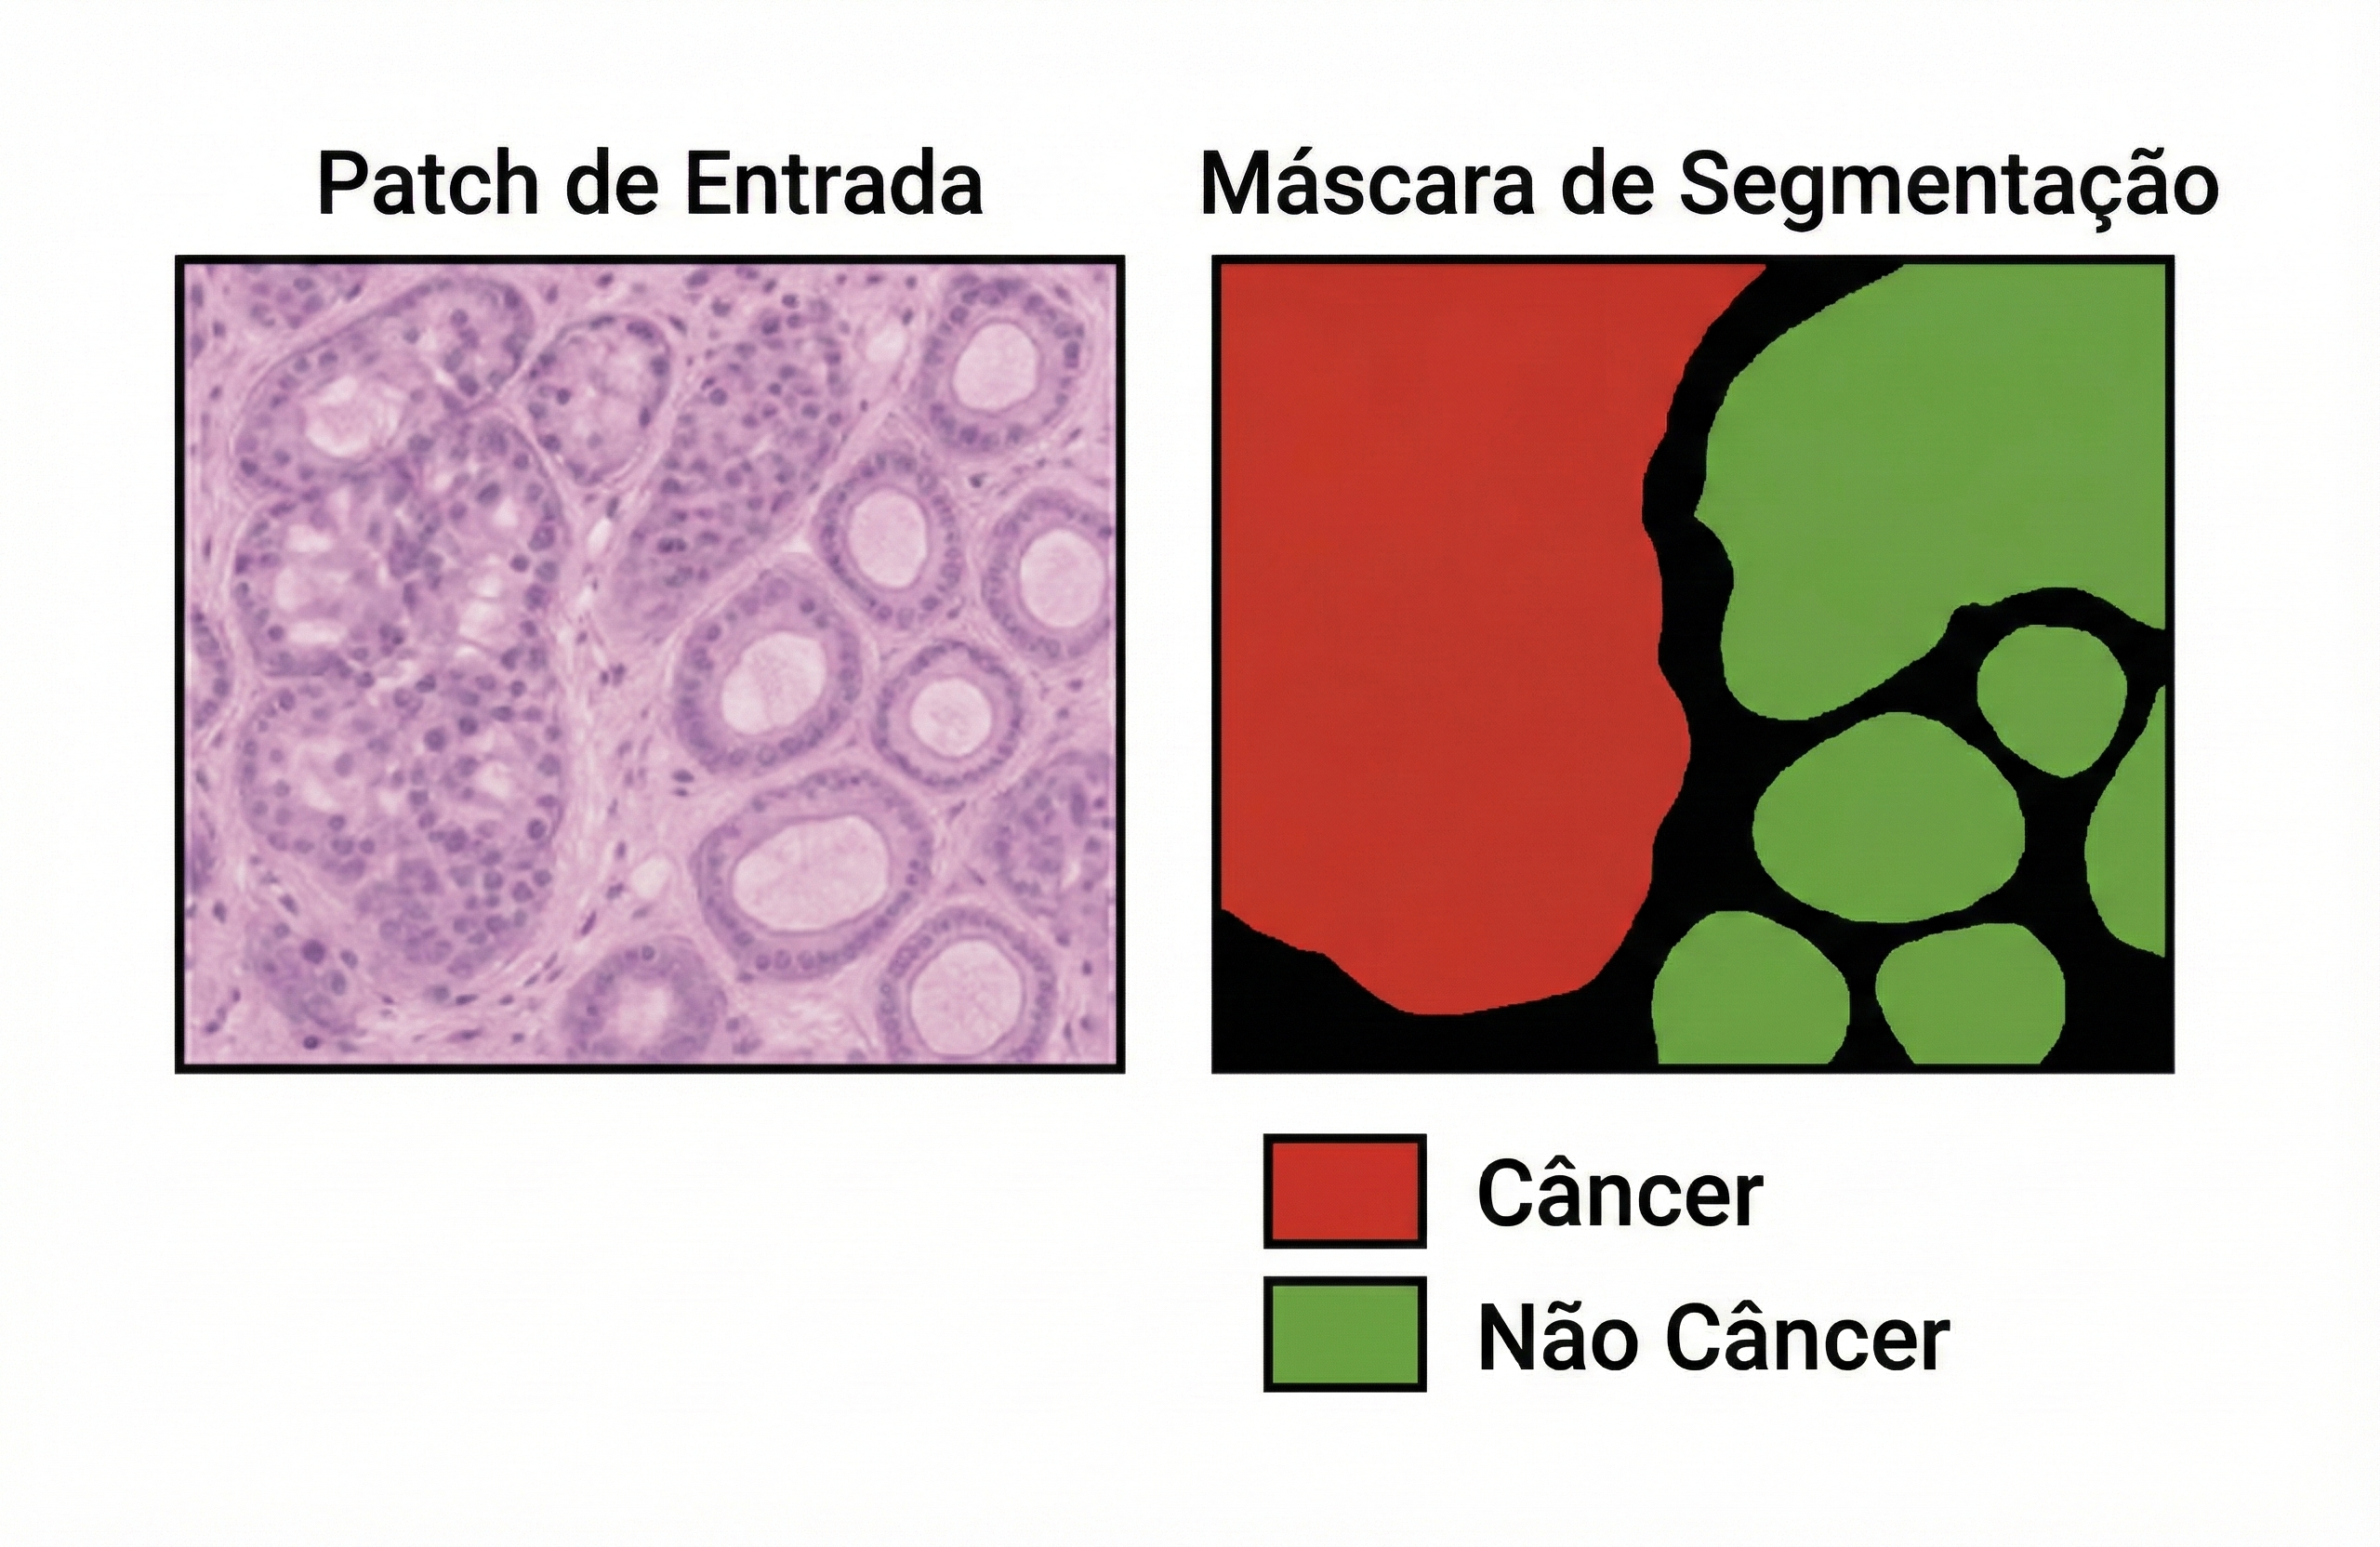
\includegraphics[width=0.85\textwidth]{figuras/semantic_segmentation.png} 
    \caption[Exemplo de Segmentação Semântica em Patologia Digital]{Ilustração do conceito de segmentação semântica aplicado a um \textit{patch} de WSI de próstata corado com H\&E. \textbf{(Esquerda)} Imagem de entrada exibindo regiões com características cancerosas e não cancerosas. \textbf{(Direita)} Máscara de segmentação correspondente, onde cada pixel é classificado: vermelho para "câncer" e verde para "não câncer", demonstrando a delineação precisa das regiões conforme abordagens como as de \textcite{Long2015}. Figura gerada pelo autor utilizando ferramenta de IA.}
    \label{fig:segmentacao_semantica_exemplo} % Label descritivo para a figura
\end{figure}

\subsection{Arquiteturas de Aprendizado Profundo para Segmentação}\label{subsec:arquiteturas_dl}

Duas famílias principais de arquiteturas de DL têm se destacado em tarefas de visão computacional, incluindo a segmentação semântica em patologia digital: CNNs e \textit{Transformers} \cite{Takahashi2024}.


\subsubsection{Redes Neurais Convolucionais (CNNs)}\label{subsubsec:cnns}
As CNNs foram um marco na visão computacional, sendo introduzidas no trabalho seminal de \textcite{Krizhevsky2012} (AlexNet). Sua arquitetura é inspirada no córtex visual humano e é caracterizada pelo uso de camadas convolucionais, que aplicam filtros (\textit{kernels}) para extrair características locais das imagens; camadas de ativação não linear (\eg, \textit{Rectified Linear Unit} (ReLU)), que introduzem não linearidades essenciais para o aprendizado de padrões complexos; e camadas de \textit{pooling} (agrupamento), que reduzem a dimensionalidade espacial dos mapas de características e aumentam o campo receptivo, conferindo uma certa invariância a pequenas translações \cite{LeCun1998, Goodfellow2016}.

A \Figura{fig:cnn_arquitetura_hierarquia} ilustra de forma esquemática este processo. Uma imagem de entrada é processada sequencialmente por blocos de convolução, ativação e, opcionalmente, \textit{pooling}. As camadas convolucionais iniciais tendem a aprender características de baixo nível, como bordas, cantos e texturas simples. À medida que a informação flui através da rede, camadas mais profundas combinam essas características mais simples para detectar padrões mais complexos e abstratos, como partes de objetos ou conceitos semânticos de alto nível. Essa capacidade de aprender automaticamente uma hierarquia de características é um dos principais pontos fortes das CNNs. Após a extração de características, camadas totalmente conectadas (\textit{Fully Connected Layers}) podem ser utilizadas para realizar a tarefa final.

\begin{figure}[!htb]
    \centering
    % Substitua pelo caminho da sua NOVA imagem gerada
    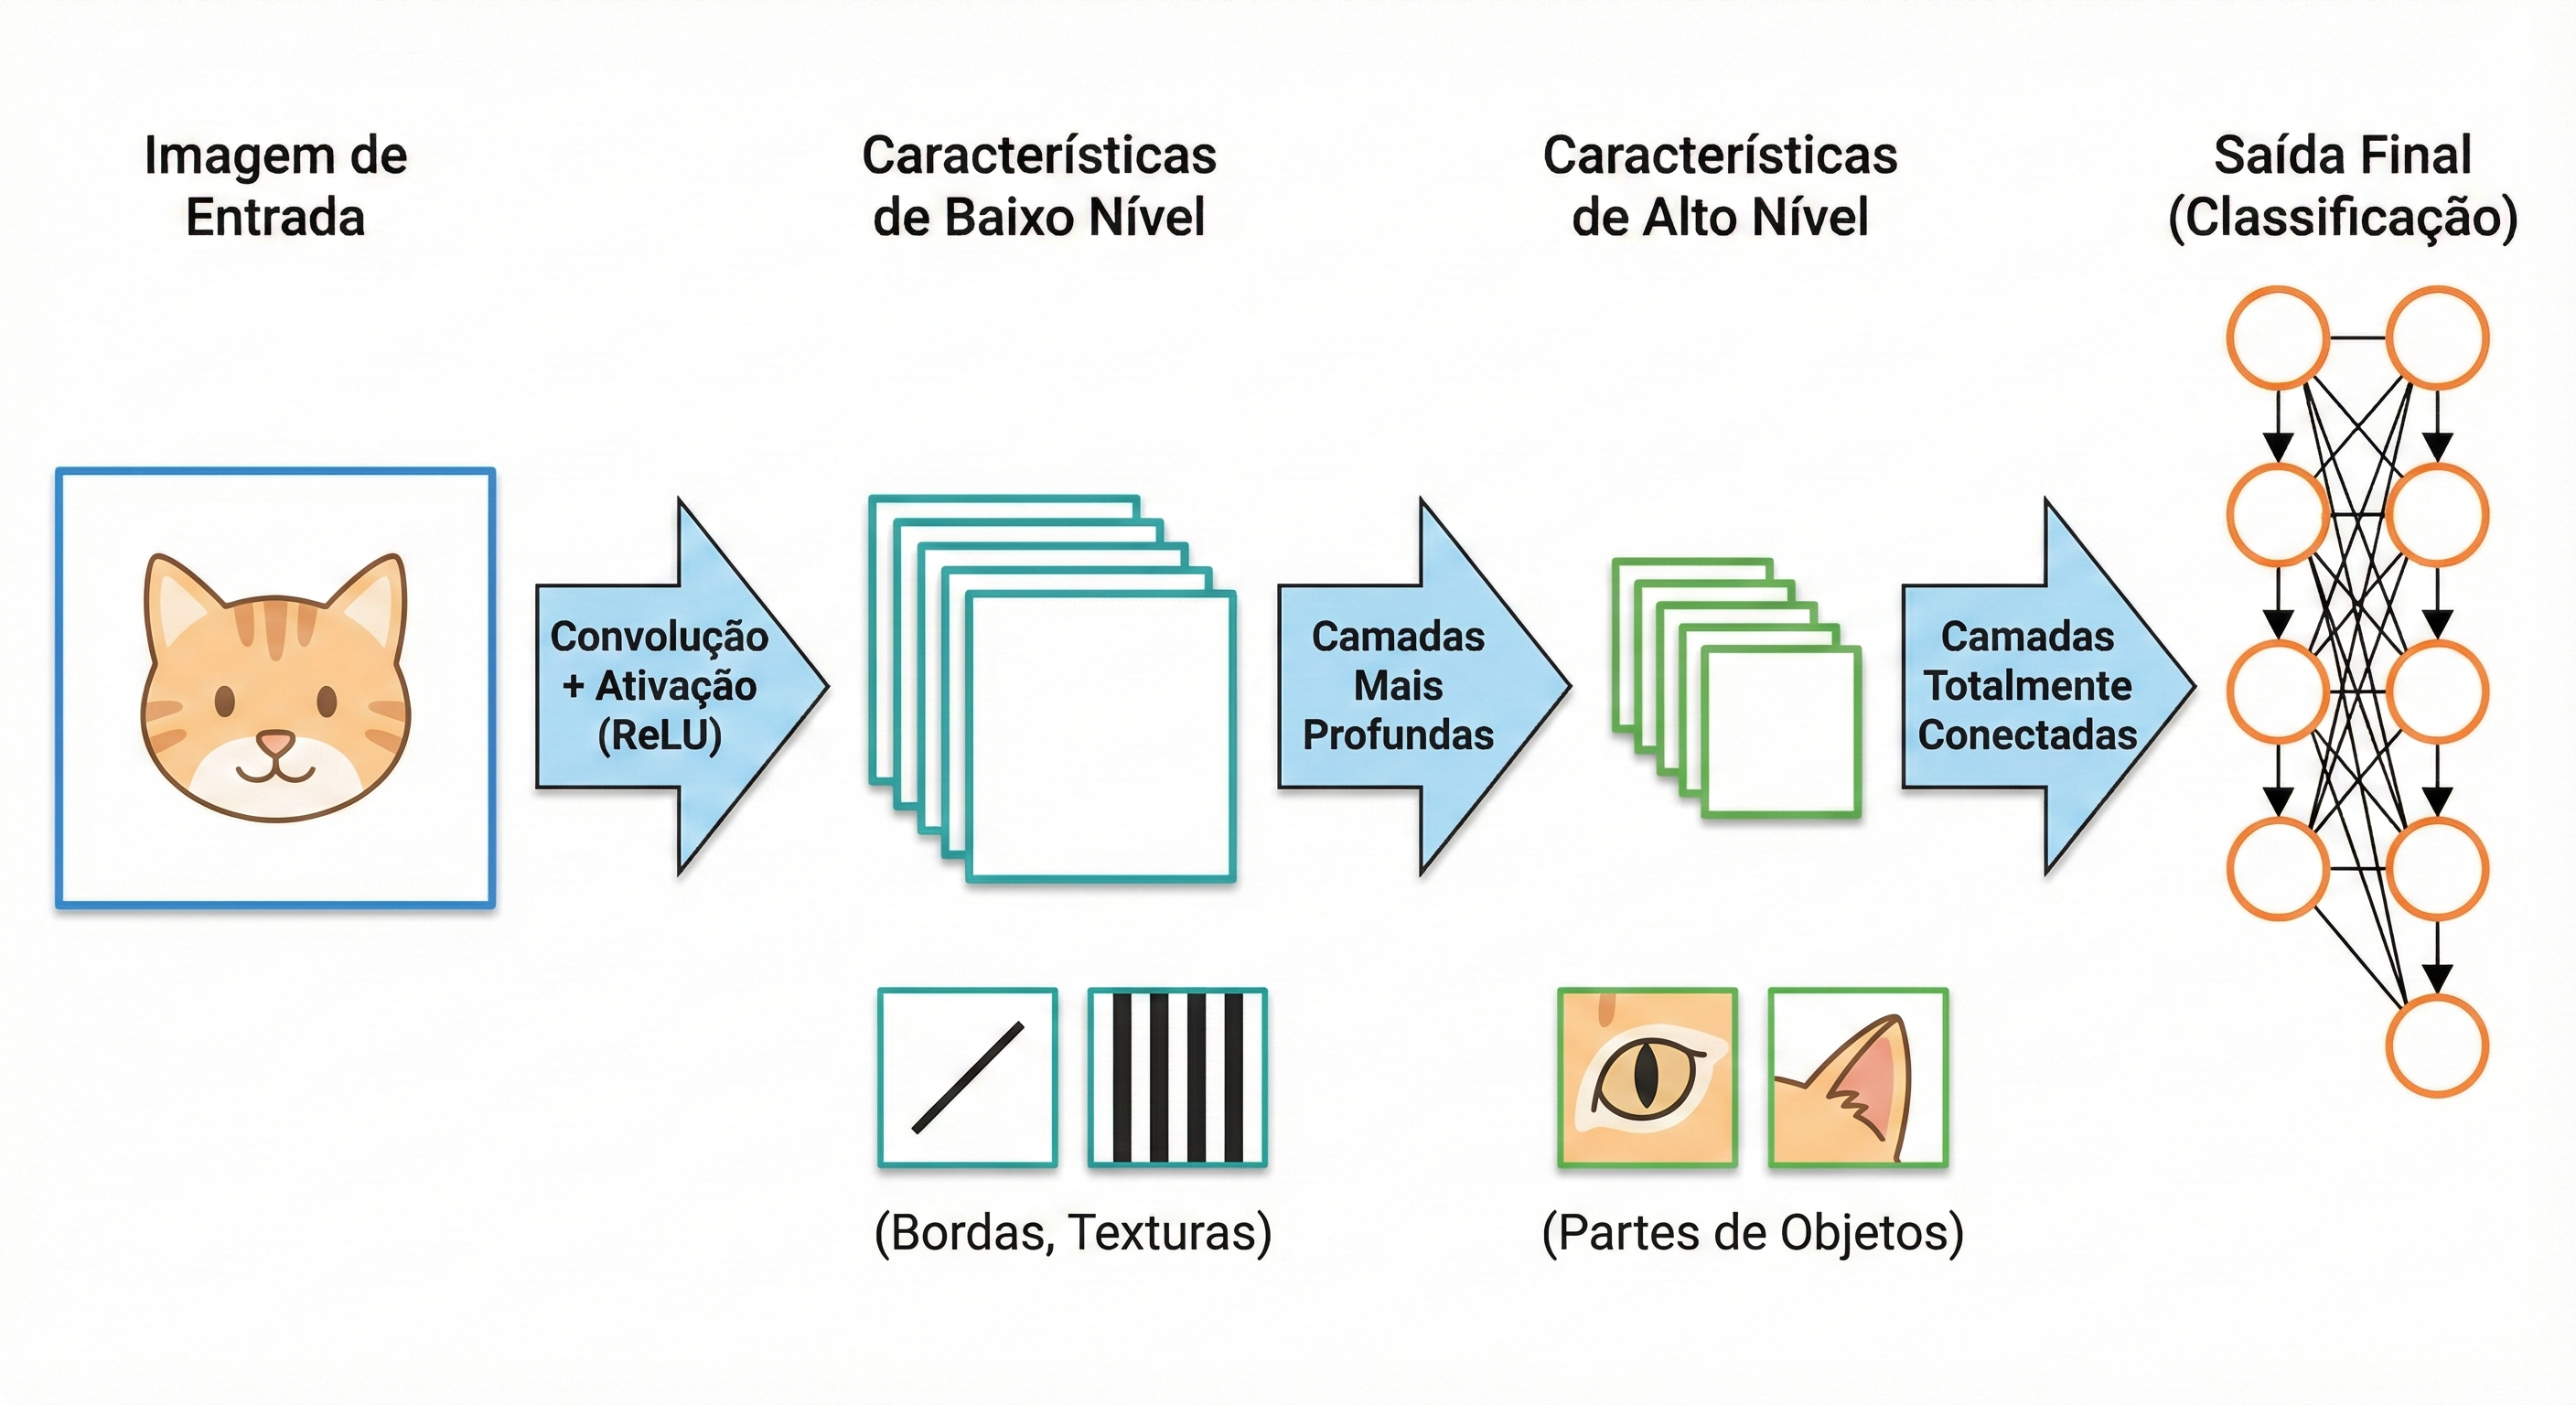
\includegraphics[width=\textwidth]{figuras/CNN.png}
    \caption[Fluxo esquemático e hierarquia de características em uma CNN.]{Representação simplificada do fluxo de processamento em uma CNN típica. A imagem de entrada passa por camadas sucessivas de convolução e ativação. As camadas iniciais detectam características simples (baixo nível, como bordas), enquanto as camadas mais profundas combinam essas informações para identificar padrões complexos e partes de objetos (alto nível), culminando nas camadas totalmente conectadas para a decisão final. Figura gerada pelo autor utilizando ferramenta de IA.}
    \label{fig:cnn_arquitetura_hierarquia}
\end{figure}


\subsubsection{\textit{Transformers} em Visão Computacional}\label{subsubsec:transformers_visao}

Originalmente propostos para tarefas de PLN \cite{Vaswani2017}, os \textbf{\textit{Transformers}} revolucionaram o campo devido ao seu mecanismo de auto-atenção (do inglês \textit{self-attention}). Este mecanismo permite modelar dependências de longo alcance entre elementos de uma sequência, capturando relações globais independentemente da distância espacial entre eles.

Fundamentalmente, o mecanismo de atenção calcula uma soma ponderada de valores, onde o peso atribuído a cada valor é determinado por uma função de compatibilidade da entrada com uma chave \cite{Vaswani2017}. Matematicamente, a operação de atenção padrão, denominada \textit{Scaled Dot-Product Attention}, recebe como entrada \textit{Queries} ($Q$), \textit{Keys} ($K$) e \textit{Values} ($V$). A saída da atenção é calculada conforme a Equação \ref{eq:attention}:

\begin{equation} \label{eq:attention}
    \textbf{\text{Attention}(Q, K, V)} = \text{softmax}\left(\frac{QK^T}{\sqrt{d_k}}\right)V
\end{equation}

\noindent onde $d_k$ representa a dimensão das chaves. O termo $QK^T$ calcula a similaridade entre as consultas e as chaves através do produto escalar, enquanto o fator de escala $\frac{1}{\sqrt{d_k}}$ é utilizado para evitar que o produto escalar cresça excessivamente em magnitude, o que poderia levar a gradientes muito pequenos durante o treinamento. A função \textit{softmax} normaliza os resultados para que somem 1, gerando os pesos de atenção que são aplicados aos valores $V$.

A adaptação dessa arquitetura para visão computacional consolidou-se notadamente com o \Sigla{\textit{Vision Transformer}}{ViT} \cite{Dosovitskiy2021}. O ViT demonstrou que os \textit{Transformers} podem alcançar desempenho competitivo ou superior às CNNs em tarefas de reconhecimento de imagem, especialmente quando pré-treinados em grandes conjuntos de dados. No ViT padrão, a imagem é tratada como uma sequência: ela é dividida em \textit{patches} (recortes) de tamanho fixo e não sobrepostos. Estes \textit{patches} são então linearmente embutidos (do inglês \textit{flattened and linearly embedded}) e processados pelos blocos \textit{Transformer} de forma análoga aos \textit{tokens} de palavras em PLN, permitindo que o modelo aprenda relações globais entre diferentes partes da imagem desde as primeiras camadas.

% Inserção da nova figura ilustrando o processo do ViT
\begin{figure}[!htb]
    \centering
    % Substitua 'figuras/vit_architecture.png' pelo nome do arquivo gerado/baixado
    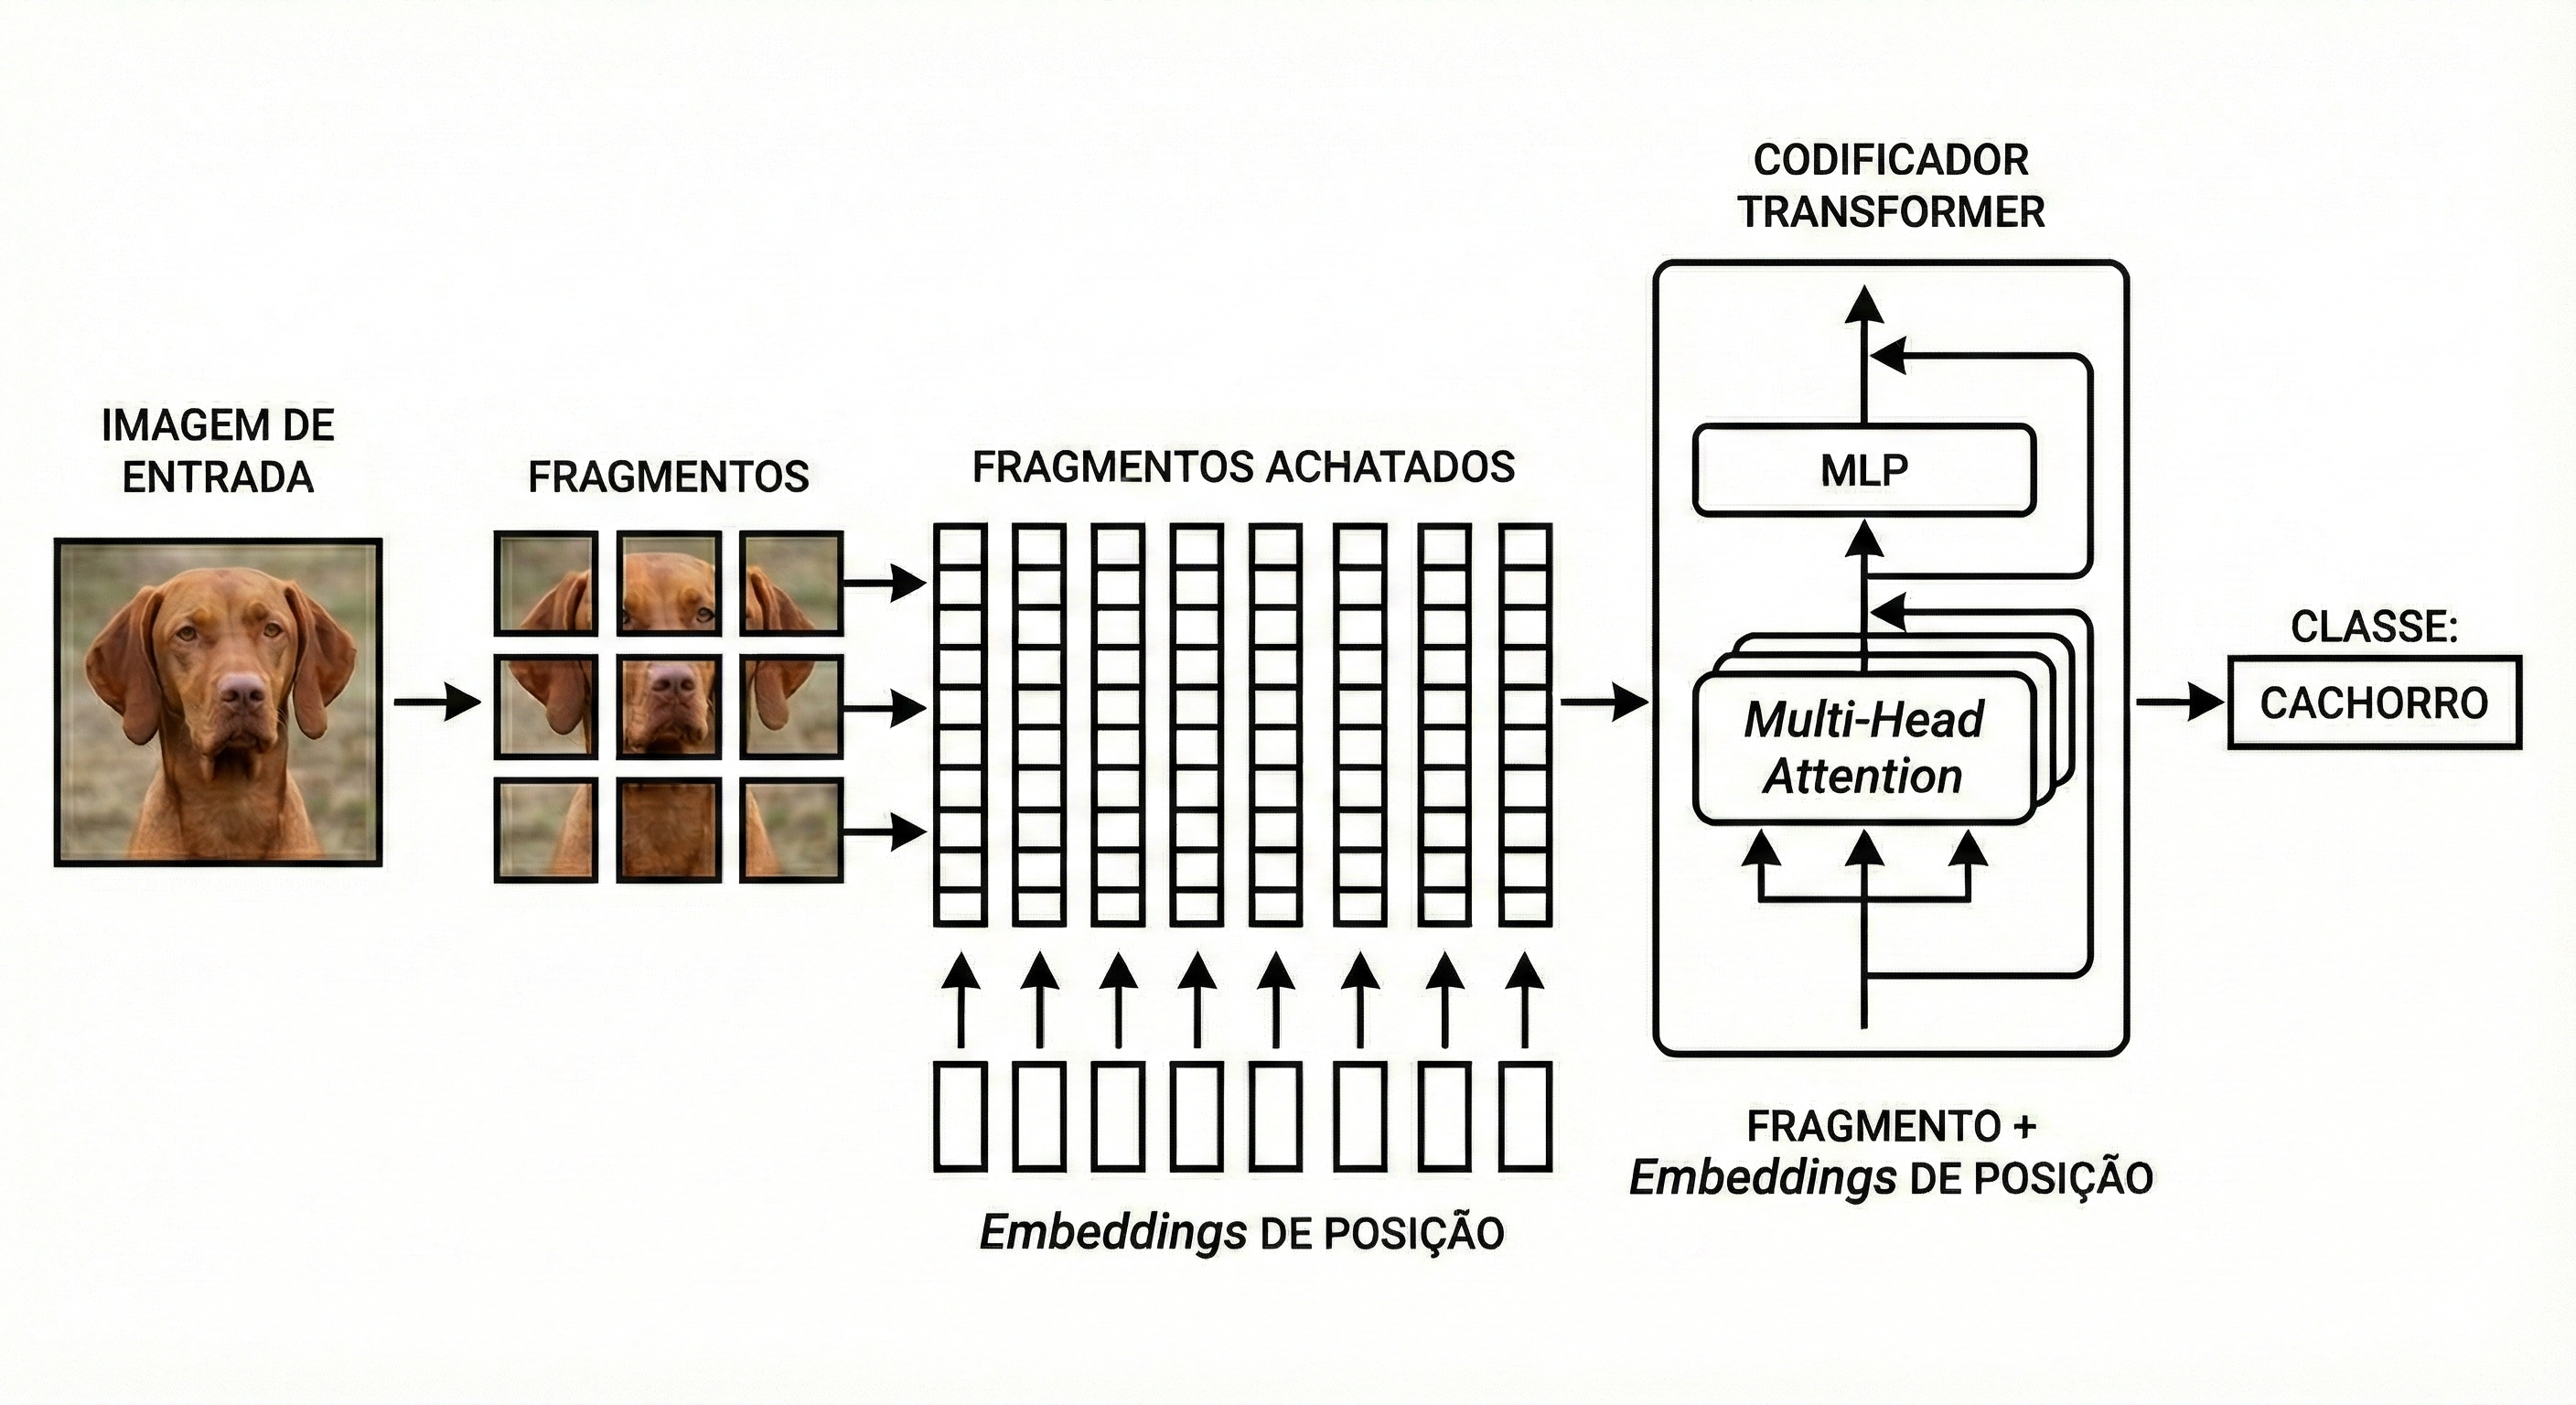
\includegraphics[width=0.9\textwidth]{figuras/vit_architecture.png}
    \caption[Esquema do Vision Transformer (ViT).]{Representação esquemática do Vision Transformer (ViT). A imagem de entrada é decomposta em uma sequência de \textit{patches} achatados. Após a projeção linear e adição de embeddings de posição, a sequência é processada por um \textit{Transformer Encoder} padrão para realizar a classificação. Figura baseada na arquitetura proposta por \textcite{Dosovitskiy2021} e gerada pelo autor utilizando ferramenta de IA.}
    \label{fig:vit_architecture}
\end{figure}

\subsection{Estratégias de Treinamento de Modelos de DL}\label{subsec:estrategias_treinamento}

O treinamento eficaz de modelos de DL para segmentação em patologia digital envolve diversas estratégias e a configuração cuidadosa de hiperparâmetros.

\subsubsection{\textit{Transfer Learning e Fine-Tuning}}\label{subsubsec:transfer_learning}
Dado que datasets médicos anotados costumam ser limitados em tamanho, o \textit{Transfer Learning} é uma técnica amplamente utilizada. Consiste em inicializar um modelo com pesos pré-treinados em um dataset de larga escala, como o ImageNet \cite{Deng2009}, que contém milhões de imagens naturais. A hipótese é que as características aprendidas em imagens naturais (\eg, bordas, texturas) são transferíveis e úteis para tarefas médicas \cite{Shin2016}. O processo de \textit{Fine-Tuning} envolve então o ajuste fino desses pesos pré-treinados utilizando o dataset específico da tarefa médica, permitindo que o modelo se adapte ao novo domínio.

\subsubsection{Aumento de Imagens}\label{subsubsec:image_augmentation}

Para aumentar artificialmente a diversidade do conjunto de treinamento e melhorar a robustez dos modelos, técnicas de Aumento de Imagens (do inglês \textit{Image Augmentation}) são comumente empregadas. A variabilidade de coloração, em particular, é um dos maiores desafios em patologia computacional. Conforme demonstrado por \textcite{TELLEZ2019101544}, a aplicação de \textit{augmentation} que simula variações de coloração é uma estratégia eficaz para criar redes neurais mais invariantes a essas mudanças, melhorando a generalização entre diferentes laboratórios e scanners.

Neste trabalho, conforme detalhado na \Secao{sec:metodologia_augmentation}, utilizamos uma combinação de transformações (gerais e específicas para o domínio) \cite{Shorten2019}. A \Figura{fig:exemplos_augmentation_atualizada} ilustra o \textit{patch} original e seis exemplos das variações geradas: Transformações geométricas como \textbf{Rotação Horizontal} (do inglês \Sigla{\textit{Horizontal Flip}}{HF}), \textbf{Rotação Vertical} (do inglês \Sigla{\textit{Vertical Flip}}{VF}) e \textbf{Rotação Aleatória} (do inglês \Sigla{\textit{Random Rotate}}{RR}); \textbf{Aplicação de ruído Gaussiano} (do inglês \Sigla{\textit{Gaussian Blur}}{GB}); e, crucialmente, \textbf{transformações no espaço de cor} \Sigla{\textit{H\&E Stain}}{HED} e \textbf{alterações de Matiz, Saturação e Valor} (do inglês \Sigla{\textit{Hue Saturation Value}}{HSV}). A aplicação sinérgica dessas transformações ajuda a mitigar o \textit{overfitting} e expõe o modelo a uma gama mais ampla e realista de variações de aparência e coloração presentes nos dados.

\begin{figure}[!htb]
    \centering
    % --- Linha 1 ---
    \begin{subfigure}[b]{0.32\textwidth}
        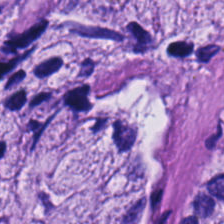
\includegraphics[width=\linewidth]{figuras/example_original.png}
        \caption{Original}
        \label{fig:aug_original_v2}
    \end{subfigure}
    \hfill
    \begin{subfigure}[b]{0.32\textwidth}
        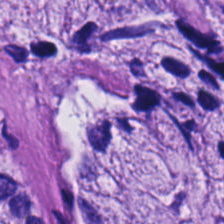
\includegraphics[width=\linewidth]{figuras/example_HF.png}
        \caption{Rotação Horiz. (HP)}
        \label{fig:aug_hp_v2}
    \end{subfigure}
    \hfill
    \begin{subfigure}[b]{0.32\textwidth}
        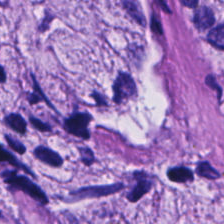
\includegraphics[width=\linewidth]{figuras/example_VF.png}
        \caption{Rotação Vert. (VF)}
        \label{fig:aug_vf_v2}
    \end{subfigure}
    
    \vspace{0.5cm} % Espaço vertical entre as linhas

    % --- Linha 2 ---
    \begin{subfigure}[b]{0.32\textwidth}
        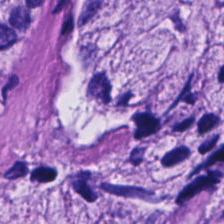
\includegraphics[width=\linewidth]{figuras/example_RR.png}
        \caption{Rotação Aleat. (RR)}
        \label{fig:aug_rr_v2}
    \end{subfigure}
    \hfill
    \begin{subfigure}[b]{0.32\textwidth}
        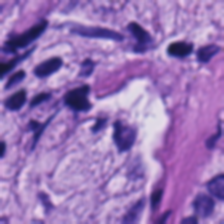
\includegraphics[width=\linewidth]{figuras/example_GB.png}
        \caption{Desfoque Gauss. (GB)}
        \label{fig:aug_gb_v2}
    \end{subfigure}
    \hfill
    \begin{subfigure}[b]{0.32\textwidth}
        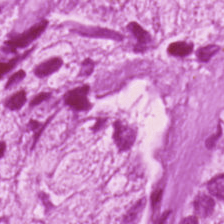
\includegraphics[width=\linewidth]{figuras/example_HED.png}
        \caption{Perturbação H\&E (HED)}
        \label{fig:aug_hed_v2}
    \end{subfigure}
    
    \vspace{0.5cm} % Espaço vertical entre as linhas

    % --- Linha 3 (Centralizada) ---
    \begin{subfigure}[b]{0.32\textwidth}
        \centering
        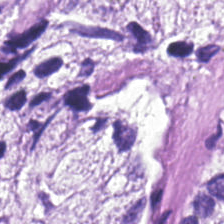
\includegraphics[width=\linewidth]{figuras/example_HSV.png}
        \caption{Alteração HSV (HSV)}
        \label{fig:aug_hsv_v2}
    \end{subfigure}

    \caption[Exemplos de Image Augmentation aplicados.]{Exemplos de técnicas de \textit{image augmentation} aplicadas a um \textit{patch} original (a). As transformações incluem: (b) Rotação Horizontal (HP), (c) Rotação Vertical (VF), (d) Rotação Aleatória (RR), (e) Desfoque Gaussiano (GB), (f) Perturbação de coloração H\&E (HED) que simula variações nos corantes, e (g) Alteração de Matiz, Saturação e Valor (HSV).}
    \label{fig:exemplos_augmentation_atualizada}
\end{figure}

\subsubsection{Otimização e Regularização}\label{subsubsec:otimizacao_regularizacao}
O treinamento de redes neurais é um problema de otimização, onde o objetivo é encontrar os pesos da rede que minimizam uma função de perda.
A \textbf{Taxa de Aprendizado (\textit{Learning Rate})} é um hiperparâmetro crucial que controla o tamanho do passo dado pelo otimizador na direção do gradiente. Uma taxa muito alta pode levar à instabilidade, enquanto uma taxa muito baixa pode resultar em convergência lenta ou estagnação em mínimos locais \cite{Goodfellow2016}. Métodos como o \textit{Learning Rate Finder} \cite{Smith2017} podem auxiliar na escolha de uma faixa inicial adequada.
As \textbf{Funções de Perda (\textit{Loss Functions})} quantificam a discrepância entre as previsões do modelo e o \textit{ground truth}. Para classificação binária, a \textit{Binary Cross-Entropy} (BCE) é uma escolha padrão \cite{Goodfellow2016}. Em tarefas de segmentação, especialmente com desbalanceamento de classes, a \textit{Dice Loss}, derivada do Coeficiente de Dice \cite{Dice1945, Milletari2016}, pode ser utilizada para maximizar diretamente a sobreposição espacial entre a predição e a máscara real. A combinação de diferentes funções de perda, como BCE e Dice Loss, pode levar a um melhor desempenho \cite{Khened2021}.
\textbf{Otimizadores}, como o AdamW \cite{Loshchilov2019} (uma variação do Adam \cite{Kingma2014} com melhor tratamento da regularização de decaimento de peso), são algoritmos que ajustam os pesos da rede com base nos gradientes calculados.
\textbf{Schedulers de Taxa de Aprendizado} ajustam dinamicamente a taxa de aprendizado durante o treinamento, por exemplo, reduzindo-a quando a perda estabiliza, para refinar a convergência. Estratégias mais recentes, como o ScheduleFree \cite{Defazio2024}, buscam automatizar esse processo.
O \textbf{Dropout} \cite{Srivastava2014} é uma técnica de regularização popular que desativa aleatoriamente uma fração de neurônios durante o treinamento, prevenindo co-adaptações complexas e melhorando a generalização.

\subsection{Métricas de Avaliação para Segmentação Semântica}\label{subsec:metricas_avaliacao}
A avaliação quantitativa do desempenho de modelos de segmentação semântica requer métricas apropriadas. Para definir essas métricas, consideramos as seguintes quantidades básicas calculadas em nível de pixel para a classe de interesse (neste caso, "câncer"):
\begin{itemize}
    \item \textbf{\Sigla{\textit{True Positives}}{TP}:} Número de \textit{pixels} corretamente classificados como pertencentes à classe de interesse.
    \item \textbf{\Sigla{\textit{True Negatives}}{TN}:} Número de \textit{pixels} corretamente classificados como \textit{não} pertencentes à classe de interesse.
    \item \textbf{\Sigla{\textit{False Positives}}{FP}:} Número de \textit{pixels} incorretamente classificados como pertencentes à classe de interesse (Erro Tipo I).
    \item \textbf{\Sigla{\textit{False Negatives}}{FN}:} Número de \textit{pixels} incorretamente classificados como \textit{não} pertencentes à classe de interesse (Erro Tipo II).
\end{itemize}


Com base nessas quantidades, as métricas utilizadas neste trabalho são:

A \textbf{Acurácia} mede a proporção geral de \textit{pixels} classificados corretamente, mas pode ser enganosa em cenários com classes desbalanceadas (onde uma classe domina a outra). É calculada como \cite{Muller2022}:
\begin{equation}\label{eq:acuracia}
    \text{Acurácia} = \frac{TP + TN}{TP + TN + FP + FN}
\end{equation}

O \textbf{Coeficiente de Dice} (do inglês \Sigla{\textit{Dice Similarity Coefficient}}{DSC}) também conhecido como \textbf{F1-Score} em nível de pixel, mede a sobreposição entre a predição e o valor real, sendo mais robusto para segmentação e desbalanceamento de classes. Varia de 0 (nenhuma sobreposição) a 1 (sobreposição perfeita). É definido como \cite{Muller2022}:
\begin{equation}\label{eq:dice}
    \text{Dice} = \frac{2 \times TP}{2 \times TP + FP + FN}
\end{equation}

A \textbf{Intersecção sobre União} (do inglês \textbf{\Sigla{\textit{Intersection over Union}}{IoU}}), também conhecida como \textbf{Índice de Jaccard}, é outra métrica de sobreposição robusta, calculando a razão entre a área de interseção e a área de união entre a predição e o valor real \cite{Taha2015}. Varia de 0 a 1 e é calculada como \cite{Muller2022}:
\begin{equation}\label{eq:iou}
    \text{IoU} = \frac{TP}{TP + FP + FN} \protect\footnote{As métricas Coeficiente de Dice e IoU estão relacionadas pela seguinte expressão: $\text{Dice} = \frac{2 \times \text{IoU}}{1 + \text{IoU}}$.}
\end{equation}

A Curva \textbf{ROC} é um gráfico que ilustra a capacidade diagnóstica de um classificador binário à medida que seu limiar de discriminação varia. Conforme visualizado na \Figura{fig:curva_roc_esquematica}, ela plota a \Sigla{\textit{True Positive Rate}}{TPR}, que é a Taxa de Verdadeiros Positivos, no eixo Y, contra a \Sigla{\textit{False Positive Rate}}{FPR}, que é a  Taxa de Falsos Positivos, no eixo X \cite{Fawcett2006}. A linha diagonal representa o desempenho de um classificador aleatório (AUC = 0.5), enquanto curvas que se arqueiam em direção ao canto superior esquerdo (0,1) indicam melhor desempenho discriminatório. O ponto (0,1) representa o classificador ideal (100\% de sensibilidade, 100\% de especificidade). A \textbf{AUC} é uma métrica escalar que resume este desempenho, variando de 0.5 (aleatório) a 1.0 (perfeito).

\begin{figure}[!htb] % O especificador [!htb] sugere fortemente ao LaTeX colocar a figura aqui, no topo ou no fundo da página atual.
    \centering
    % Comando para incluir sua imagem - substitua 'nome_arquivo_imagem_roc'
    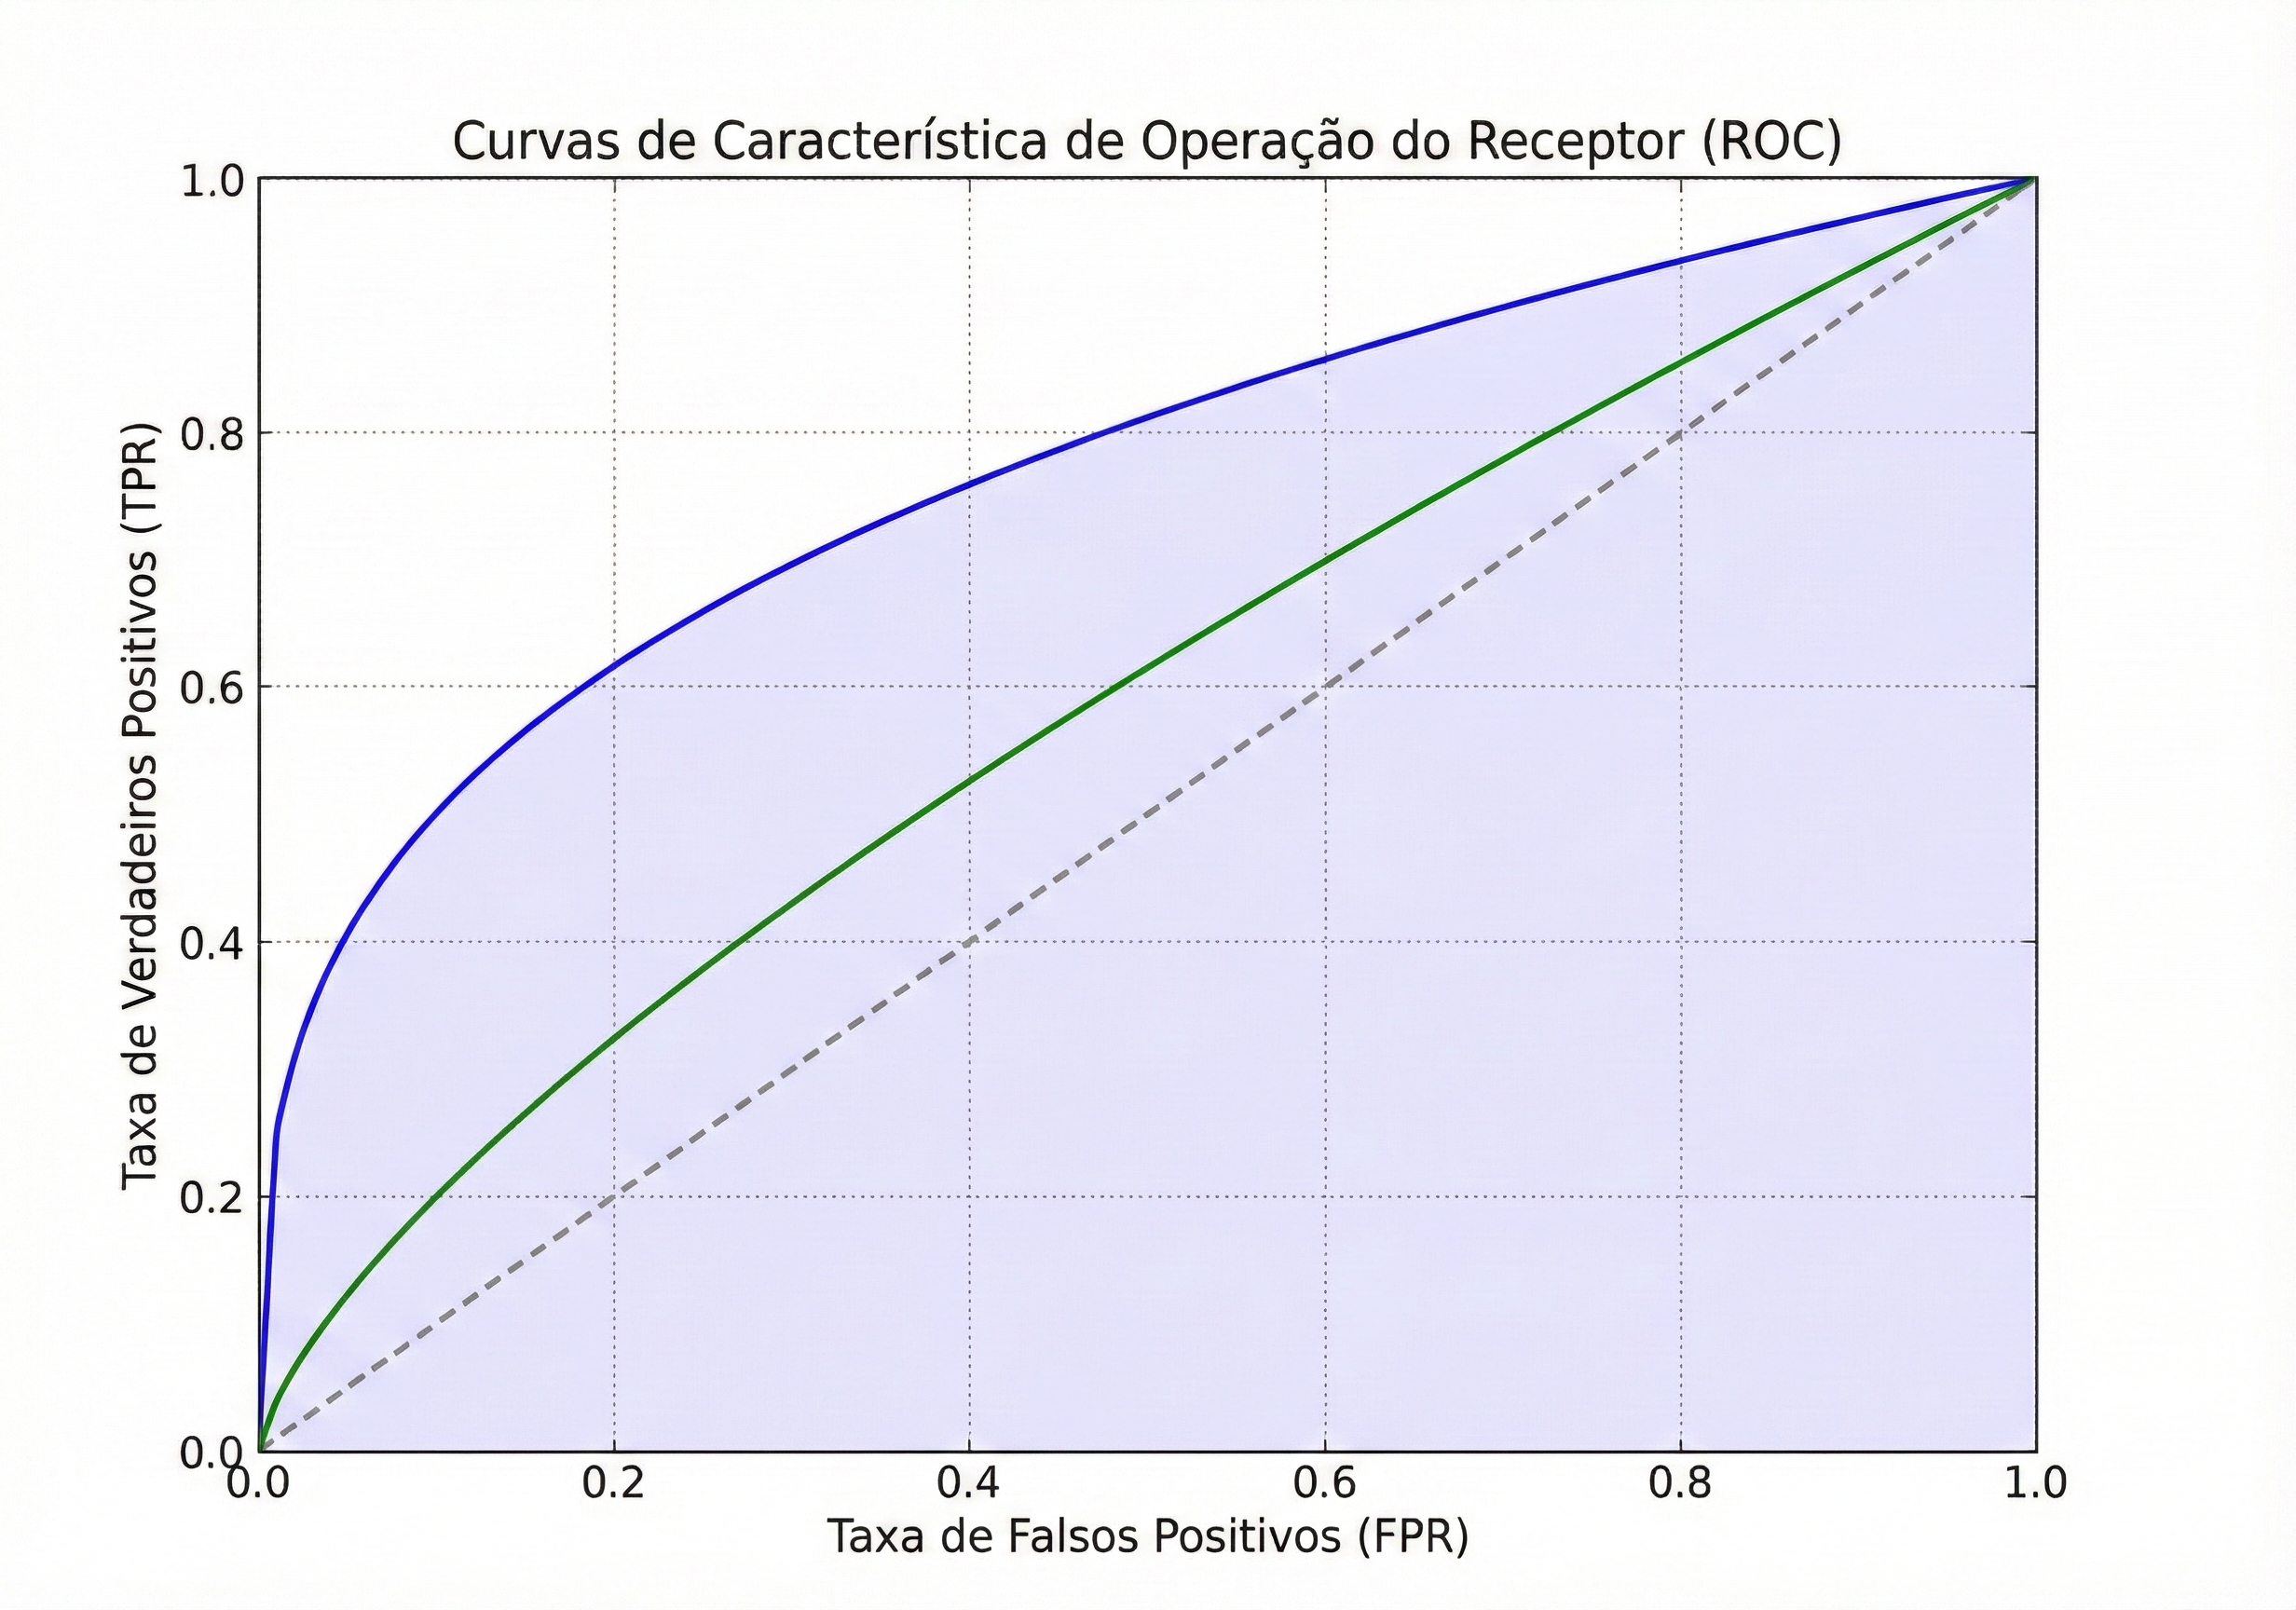
\includegraphics[width=0.7\textwidth]{figuras/roc_curve.png} 
 \caption[Curva ROC Esquemática]{Representação esquemática de Curvas ROC (\textit{Receiver Operating Characteristic}). O gráfico ilustra o desempenho de classificadores binários ao plotar a Taxa de Verdadeiros Positivos (TPR) contra a Taxa de Falsos Positivos (FPR). A linha diagonal tracejada representa um classificador aleatório (sem capacidade de discriminação). As linhas curvas acima da diagonal exemplificam modelos com diferentes níveis de desempenho; quanto mais a curva se aproxima do canto superior esquerdo (maximizando TPR e minimizando FPR), melhor é o modelo representado. Conceito conforme \textcite{Fawcett2006}. Figura gerada pelo autor utilizando ferramenta de IA.}
    \label{fig:curva_roc_esquematica} 
\end{figure}

A \textbf{TPR}, também conhecida como Sensibilidade (do inglês \textit{Sensitivity}) ou Revocação (dp inglês \textit{Recall}), mede a proporção de positivos reais que foram corretamente identificados \cite{Altman1994, Fletcher2014}.
\begin{equation}\label{eq:tpr}
    \text{TPR (\textit{Sensitivity})} = \frac{TP}{TP + FN}
\end{equation}

A \textbf{\Sigla{\textit{True Negative Rate}}{TNR}}, que é a Taxa de Verdadeiros Negativos, também conhecida como Especificidade (do inglês \textit{Specificity}), mede a proporção de negativos reais que foram corretamente identificados \cite{Altman1994, Fletcher2014}.
\begin{equation}\label{eq:tnr}
    \text{TNR (\textit{Specificity})} = \frac{TN}{TN + FP}
\end{equation}

Complementar à TNR, a \textbf{FPR}, que é utilizada como eixo horizontal na Curva ROC, mede a proporção de negativos reais que foram incorretamente classificados como positivos. É calculada como:
\begin{equation}\label{eq:fpr}
    \text{FPR} = \frac{FP}{TN + FP} = 1 - \text{TNR}
\end{equation}

A \textbf{Precisão} (do inglês \textit{Precision}) avalia a proporção de instâncias classificadas como positivas que são, de fato, verdadeiras positivas. É particularmente importante quando o custo de um falso positivo é alto \cite{Powers2011, Hastie2009}.
\begin{equation}\label{eq:precisao}
    \text{\textit{Precision}} = \frac{TP}{TP + FP}
\end{equation}

A seleção e análise conjunta dessas métricas fornecem uma avaliação abrangente do desempenho dos modelos de segmentação desenvolvidos neste trabalho.

\subsection{\textit{Ensembles} de Modelos}\label{subsec:ensembles}
Técnicas de \textit{Ensemble Learning} combinam as previsões de múltiplos modelos para obter um desempenho geral melhor e mais robusto do que qualquer modelo individual \cite{Dietterich2000}. Métodos comuns incluem \textit{bagging}, \textit{boosting} e \textit{stacking}. Em DL, uma abordagem simples e eficaz é a média das probabilidades preditas por diferentes modelos (para regressão ou classificação probabilística) ou a votação majoritária (para classificação). A diversidade entre os modelos no ensemble é um fator chave para seu sucesso.

\subsection{Ferramentas Computacionais e Hardware}\label{subsec:ferramentas_hardware}
O desenvolvimento e treinamento de modelos de DL para patologia digital demandam um ecossistema de ferramentas e hardware específico.
Linguagens de programação como \textbf{Python} são predominantes devido à sua vasta gama de bibliotecas para ciência de dados e aprendizado de máquina. \textit{frameworks} de DL como \textbf{PyTorch} \cite{Paszke2019} e TensorFlow/Keras oferecem flexibilidade e eficiência para construir e treinar redes neurais.
Bibliotecas especializadas como \textbf{OpenCV} \cite{Bradski2000} para processamento de imagem, \textbf{OpenSlide} \cite{OpenSlide} para leitura de WSIs, \textbf{Shapely} para manipulação de geometrias (útil para processar anotações XML), e bibliotecas como \textbf{Segmentation Models Pytorch} \cite{Iakubovskii2019} e \textbf{Timm} \cite{rw2019timm} que fornecem implementações de arquiteturas populares, são essenciais.
Ferramentas de monitoramento de experimentos como \textbf{AIM Stack} \cite{Arakelyan2020} auxiliam no rastreamento de métricas e comparação de execuções. A ferramenta permite o acompanhamento em tempo real de curvas como \textit{Loss}, Dice e IoU para diferentes execuções (experimentos ou \textit{folds}), facilitando a análise comparativa e a gestão do processo de treinamento.

\begin{figure}[!htb] 
    \centering
    % Comando para incluir sua imagem AIM Stack
    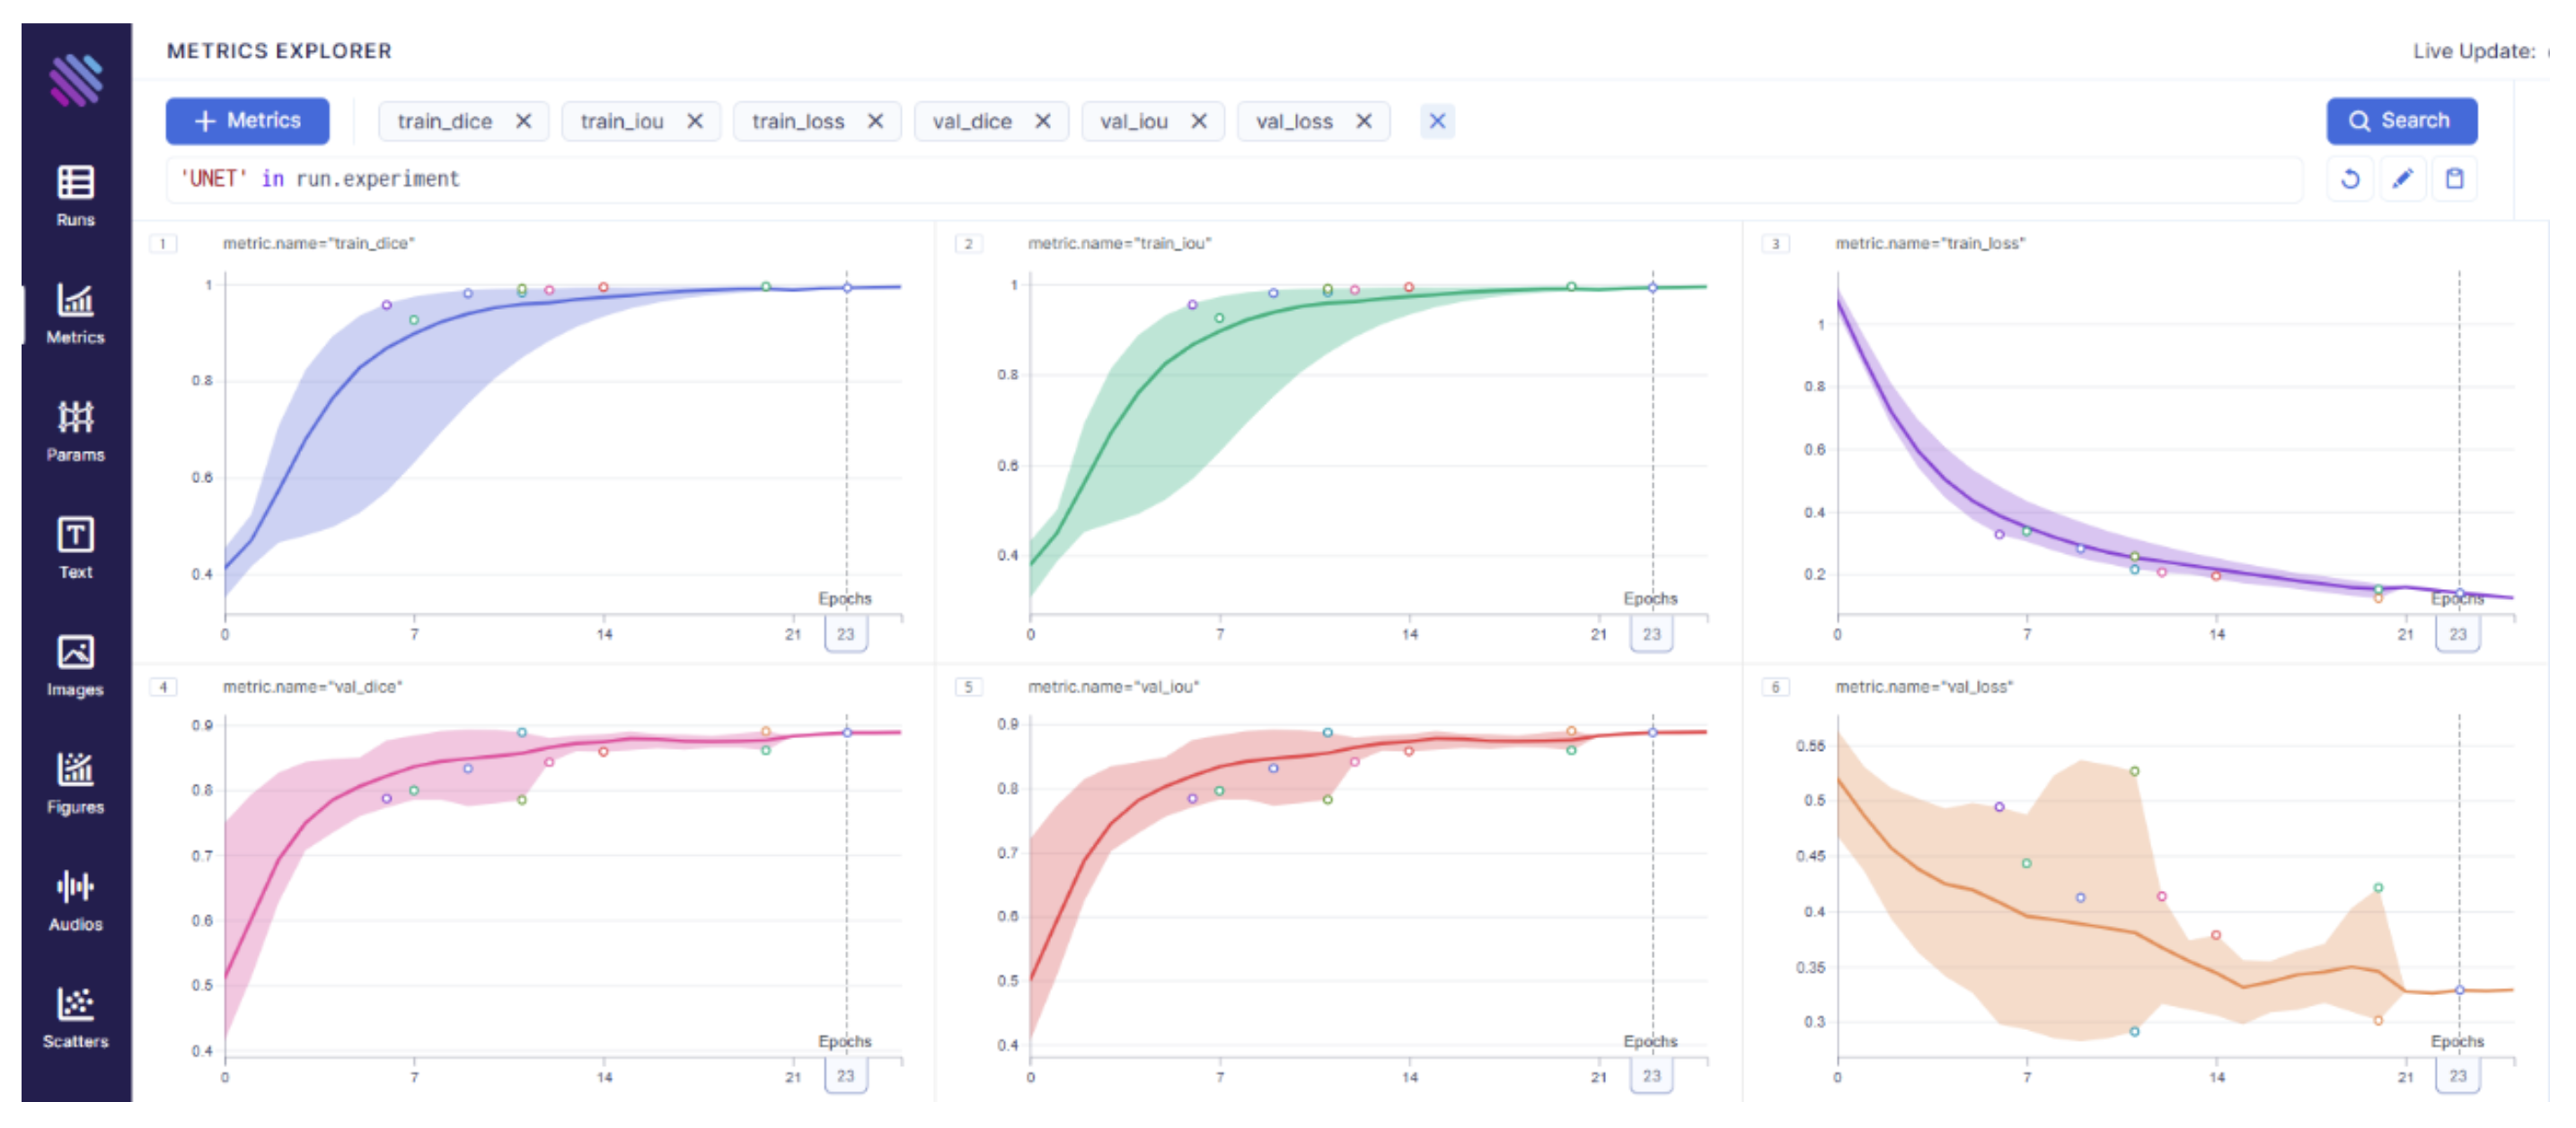
\includegraphics[width=1.0\textwidth]{figuras/AIM_stack.png} % Ajuste a largura conforme necessário
    \caption[Interface do AIM Stack para Monitoramento]{Exemplo da interface da plataforma AIM Stack utilizada para monitoramento e visualização das métricas de treinamento e validação dos modelos de DL.\textcite{Arakelyan2020}.}
    \label{fig:aim_stack_interface} % Novo label para esta figura
\end{figure}

O treinamento de modelos de DL é computacionalmente intensivo, tornando o uso de \Sigla{\textit{Graphics Processing Units}}{GPU} indispensável para acelerar os cálculos. Plataformas baseadas em nuvem como \textbf{Google Colab} oferecem acesso a GPUs, facilitando a experimentação e o treinamento, especialmente para pesquisadores com recursos locais limitados.

% Continuando o Capítulo 2...

\section{Trabalhos Relacionados}\label{sec:trabalhos_relacionados}

Diante da vasta produção científica na área, esta seção apresenta uma análise de trabalhos representativos, discutindo abordagens metodológicas, arquiteturas e frameworks computacionais. Este levantamento visa contextualizar a presente dissertação e delinear as lacunas específicas que este trabalho busca mitigar.

Para fundamentar esta análise, foi conduzida uma revisão da literatura com o objetivo de identificar e avaliar \textit{frameworks} baseados em DL aplicados à segmentação de WSIs em biópsias de câncer de próstata. O processo seguiu as diretrizes do método PRISMA (\textit{Preferred Reporting Items for Systematic Reviews and Meta-Analyses}) \cite{Moher2009}, complementado por uma seleção discricionária de artigos adicionais relevantes para componentes-chave da pesquisa.

O protocolo da revisão iniciou-se com a definição dos critérios de elegibilidade. A população de interesse foi definida como estudos que abordam \textit{frameworks} computacionais completos para o processamento de WSIs de câncer de próstata. A intervenção de interesse foi delimitada a \textit{frameworks} baseados em DL que englobassem o pipeline desde o pré-processamento das imagens até o pós-processamento dos resultados de segmentação, incluindo métodos para detecção de tecido e treinamento de modelos. Os comparadores abrangeram variações nos componentes dos \textit{pipelines}, como diferentes técnicas de normalização de cor, estratégias de seleção de \textit{patches} e arquiteturas de modelos. Os desfechos primários foram a descrição da metodologia do \textit{framework}, sua completude (end-to-end), eficiência, e replicabilidade.

Foram estabelecidos critérios objetivos de inclusão e exclusão. Incluíram-se estudos que: (1) apresentassem avaliação de processos compostos por múltiplas etapas; (2) fornecessem análise quantitativa dos componentes do pipeline no contexto do câncer de próstata; (3) fossem artigos revisados por pares; (4) estivessem redigidos em inglês; e (5) fossem publicados em periódicos científicos ou anais de conferências de reconhecida relevância. Foram excluídos estudos: (1) limitados à investigação de componentes isolados (como apenas funções de perda ou técnicas de aumento de dados) sem integração em um pipeline completo; (2) que não tratassem especificamente do câncer de próstata em WSIs; ou (3) que apresentassem lacunas metodológicas significativas ou não detalhassem suficientemente o \textit{framework} para permitir uma análise crítica.

A busca bibliográfica foi realizada em três bases de dados científicas: PubMed \cite{PubMed2024}, IEEE Xplore \cite{IEEEXplore2024}  e Portal de Periódicos CAPES \cite{PeriodicosCAPES2024}. As estratégias de busca foram desenvolvidas combinando termos relacionados ao câncer de próstata, WSIs e DL, com palavras-chave indicativas de \textit{pipelines} de processamento, todas em inglês. A \textit{query} de busca principal utilizada foi:
\begin{quote}
\texttt{("\textit{prostate cancer}" OR "\textit{prostatic neoplasms}" OR "\textit{prostate adenocarcinoma}") AND ("\textit{whole slide imaging}" OR "WSI" OR "\textit{digital pathology}" OR "\textit{virtual microscopy}") AND ("\textit{semantic segmentation}" OR "\textit{image segmentation}" OR "\textit{tumor segmentation}" OR "\textit{cancer segmentation}") AND ("\textit{deep learning}" OR "\textit{convolutional neural network}" OR "CNN" OR "\textit{transformer}" OR "U-Net") AND ("\textit{pipeline}" OR "\textit{framework}" OR "\textit{workflow}" OR "\textit{end-to-end}" OR "\textit{computer-aided diagnosis}" OR "CAD \textit{system}")}
\end{quote}
O recorte temporal da busca abrangeu publicações entre os anos de 2015 e 2025 (data de previsão de conclusão da busca no momento do planejamento), visando incorporar tanto estudos clássicos quanto os mais recentes e pertinentes ao escopo da revisão.

A busca inicial retornou 5 artigos no portal IEEE Xplore, 17 artigos no PubMed e 28 resultados no Portal CAPES, totalizando 50 artigos potencialmente relevantes. Após a remoção de 6 duplicatas, restaram 44 artigos únicos. Estes foram submetidos a uma triagem por título e resumo, seguida pela leitura completa dos artigos selecionados para avaliação de elegibilidade conforme os critérios de inclusão e exclusão definidos. Deste processo, apenas 6 artigos atenderam integralmente aos critérios para inclusão na análise focada em \textit{frameworks} completos. Estes estudos selecionados, juntamente com outros artigos que abordam componentes-chave relevantes para o desenvolvimento de \textit{frameworks}, são discutidos nas subseções seguintes.

\subsection{Abordagens de DL para Análise de WSIs de Câncer de Próstata}\label{subsec:dl_abordagens_wsi}

As CNNs foram pioneiras na aplicação de DL para análise de WSIs, demonstrando capacidade de aprender características hierárquicas diretamente dos dados de imagem para tarefas como classificação de \textit{patches}, detecção de mitoses e segmentação de regiões tumorais \cite{Ciresan2012, Litjens2017}. No contexto específico do câncer de próstata, as CNNs têm sido empregadas para identificar padrões de Gleason e delinear áreas cancerosas. Por exemplo, estudos iniciais focaram na classificação de \textit{patches} individuais extraídos de WSIs como benignos ou malignos, ou na atribuição de escores de Gleason \cite{Bulten2022}. % Exemplo de citação genérica sobre CNNs para Gleason.

Com a emergência dos \textit{Transformers} em visão computacional \cite{Dosovitskiy2021}, novas arquiteturas começaram a ser exploradas. A capacidade dos Transformers de modelar relações de longo alcance nos dados, através de mecanismos de atenção, oferece um contraponto às CNNs, que são inerentemente mais focadas em características locais. Essa complementaridade tem motivado o desenvolvimento de modelos híbridos CNN-Transformer, buscando combinar o melhor de ambas as abordagens para tarefas complexas \cite{10326274}.

Para tarefas mais complexas como a graduação de Gleason, que requer a identificação e quantificação de múltiplos padrões arquiteturais, arquiteturas de detecção de objetos como o Path R-CNN foram propostas \cite{Li2021PathRCNN}. % Nota: Preciso de um BibTeX para "Li et al. com o Path R-CNN". Vou criar uma chave placeholder.
O Path R-CNN demonstrou a viabilidade de realizar simultaneamente a detecção de células epiteliais e a graduação de Gleason, alcançando um desempenho notável (AUC 0,998, acurácia 89,4\%). No entanto, o foco principal de tais trabalhos reside frequentemente na inovação  da arquitetura, sem detalhar extensivamente um \textit{frameworks} de pré e pós-processamento generalizável ou estratégias para otimização e eficiência computacional.

Outros estudos concentram-se na segmentação semântica de regiões histológicas. Trabalhos como o que explora o Ensemble EfficientNetB2 U-Net \cite{Ikromjanov2023}
demonstram a eficácia de codificadores pré-treinados e técnicas de ensemble para segmentar diferentes componentes teciduais, alcançando altos escores de Coeficiente de Dice (DC) (0,891) e Intersection over Union (IoU) (0,811). Similarmente, \cite{Hassan2021}
explora modificações arquiteturais como dilatação híbrida e decomposição hierárquica para melhorar a extração de padrões de Gleason, resultando em melhorias de 3,22\% em IoU e 6,91\% em F1-score. Essas pesquisas avançam as técnicas de segmentação, mas frequentemente tratam o pipeline de processamento como um meio para validar a arquitetura, e não como o objeto central da investigação metodológica.

\subsection{\textit{Frameworks} e \textit{Pipelines} Completos em Patologia Digital}\label{subsec:frameworks_pipelines_patologia}

Reconhecendo a necessidade de soluções mais integradas, alguns pesquisadores têm se dedicado ao desenvolvimento de \textit{frameworks} e \textit{pipelines} computacionais mais completos para a análise de WSIs. O trabalho de \textcite{Khened2021} é um exemplo notável, propondo um \textit{framework} generalizado baseado em DL que abrange desde o pré-processamento e segmentação via um modelo \textit{ensemble} (combinando DenseNet-121, Inception-ResNet-V2 e DeeplabV3Plus), até a inferência eficiente com \textit{patches} sobrepostos e estimativa de incerteza %[cite: 15, 16].

A generalidade e eficácia deste \textit{framework} foram validadas quantitativamente em três desafios distintos. No dataset CAMELYON17, para câncer de mama \cite{bandi2019detection}, a abordagem de \textit{ensemble} para classificação de metástases alcançou um \textit{score} Cohen's Kappa de 0.9090, posicionando-se em terceiro lugar no \textit{leaderboard}.
Para a segmentação em DigestPath 2019, para câncer de cólon \cite{DA2022102485}, o método obteve um coeficiente Dice de 0.782.
Já no desafio PAIP 2019, para câncer de fígado, \cite{KIM2021101854}, o \textit{framework} atingiu um índice Jaccard de 0.750 na segmentação de tumor viável.
Contudo, o \textit{ensemble} proposto por \textcite{Khened2021} tem natureza puramente convolucional.

O desafio de adquirir dados anotados em larga escala é uma barreira significativa. Abordagens como a de \cite{Hassan2022}
utilizam distilação de conhecimento e aprendizado incremental para segmentar instâncias de Gleason com dados limitados, superando \textit{baselines} em IoU (2,01\%) e F1 (9,69\%). Embora cruciais para a viabilidade de \textit{frameworks} em cenários com restrição de dados, essas técnicas precisam ser integradas em um fluxo de trabalho completo e eficiente.

A questão da generalização e robustez a variações entre diferentes fontes de dados (\textit{domain shift}) é crítica para a aplicabilidade clínica. O estudo de \cite{Bulten2022}
foca explicitamente em aprender características independentes de domínio, validando a robustez do sistema em múltiplas bases (acurácia até 89,4\%). A construção de \textit{frameworks} robustos exige a incorporação sistemática dessas estratégias de generalização.

A explicabilidade e interpretabilidade dos modelos de DL também são importantes para sua aceitação na prática clínica. O HistoEM \cite{Ferrero2024}
se destaca por propor um \textit{workflow} alinhado à prática patológica, utilizando histogramas de características para classificação de glândulas e empregando Grad-CAM \cite{Selvaraju2017GradCAM} para visualização e interpretabilidade, confirmando o uso de padrões nucleares. Embora o desenvolvimento de mecanismos de explicabilidade dedicados, como os baseados em mapas de ativação, não tenha sido o foco primário da implementação inicial deste \textit{framework}, reconhece-se sua importância intrínseca e a necessidade de explorá-los em trabalhos futuros para aumentar a confiança e a utilidade clínica da ferramenta.

\subsection{Identificação da Lacuna e Posicionamento da Pesquisa}\label{subsec:lacuna_posicionamento}

A revisão da literatura revela um progresso substancial no desenvolvimento de arquiteturas de DL e técnicas específicas para análise de WSIs de câncer de próstata. No entanto, percebe-se uma carência de estudos que documentem e validem \textit{frameworks} metodológicos completos sob a perspectiva da replicabilidade e abordagem \textit{end-to-end} sistemática. Muitos artigos focam intensamente na novidade arquitetural ou na superação de métricas em \textit{benchmarks} específicos, sem detalhar exaustivamente as etapas de pré-processamento, estratégias de treinamento otimizadas para recursos limitados, ou fornecer um pipeline de código aberto e bem documentado que facilite a reprodução e adaptação por outros pesquisadores.

É neste cenário que a presente dissertação se insere. O objetivo central não é apenas propor mais uma arquitetura – embora explore a combinação sinérgica de CNNs e \textit{Transformers} – mas sim desenvolver e validar um \textit{framework} metodológico que seja:
\begin{itemize}
    \item \textbf{End-to-End:} Cobrindo todas as etapas, desde a leitura e pré-processamento da WSI até a segmentação final e inferência.
    \item \textbf{Eficiente:} Projetado considerando restrições de custo e tempo computacional, visando ser rápido e acessível (\eg, utilizando recursos como \textit{Google Colab Pro}).
    \item \textbf{Replicável:} Detalhado e documentado (com código aberto) para permitir fácil reprodução e adaptação por outros grupos de pesquisa.
    \item \textbf{Sistemático:} Oferecendo um processo estruturado e modular para abordar a segmentação de câncer de próstata em patologia digital.
\end{itemize}

Ao focar na metodologia, este trabalho busca preencher a lacuna existente, oferecendo não apenas resultados de segmentação, mas um processo robusto e acessível que possa servir de base e catalisador para futuras investigações na área. A proposta de integrar CNNs, para captura eficiente de características locais, e \textit{Transformers}, para modelagem de contexto global, dentro de um \textit{framework} sistemático e otimizado, visa alavancar os avanços técnicos demonstrados pela literatura em um contexto de maior rigor metodológico e praticidade.
